\chapter{Laser-electron interaction in vacuum}
\label{Laser-electron interaction in vacumm}
\minitoc

\dominitoc

\minitoc

\thispagestyle{empty}

\section{Ponderomotive force and electron motion in vacuum}\label{section:Ponderomotive force and electron motion in vacuum}


When electrons are accelerated away from the plasma, they do not propagate ballistically in vacuum immediately since they keep interacting with the driving laser reflecting at the plasma surface. In this section, we will describe the nature of this interaction, and in particular distinguish between the so-called "ponderomotive" regime, where electrons are expelled from high-intensity regions of the laser and the "non-ponderomotive" regime which we will describe hereafter. The Lawson-Woodward theorem states that a free charged particle cannot acquire energy from a plane wave. However, the hypotheses for this theorem to be valid are~\cite{LWtheoremLS}:
\begin{enumerate}
\item The laser propagates in vacuum without boundaries
\item The electron is relativistic in the direction of propagation $v_z\approx c$
\item No static E or B are present
\item non linear forces (such as the ponderomotive force) are neglected
\end{enumerate}
In the present context of strongly focused ultra-short laser pulses, all these hypotheses are violated such that electron acceleration is not forbidden by theory.

\subsection{Classical ponderomotive force derivation}

The ponderomotive force is a local force proportional to the average acceleration of one electron during one laser period. The existence of this force is the consequence of an inhomogeneous spatial profile of the field envelope as opposed to non-physical plane waves. If we picture an electron oscillating at the center of a Gaussian beam: (i) During one half period, the electron will accelerate in one direction of space. (ii) The electron is now located in the region of lower field strength so it will be less decelerated when regaining its original position. (ii) On average over one optical cycle, the electron will have moved from the high-intensity to  low intensity region of the beam. \\



\noindent The starting point, as usual, is the equation of motion of an electron given in a electromagnetic given field which we linearized at position $r_e^{(0)}$.

%\underbrace{\frac{dv_e^{(0)}}{dt}}_{drift}+\underbrace{\frac{dv_e^{(1)}}{dt}}_{fast motion}=-\frac{e}{m_e}(\underbrace{E(x_e^{(0)},t)}_{homogeneous field} + \underbrace{x_e^{(1)}\nabla E(x_e^{(0)}}_{drift}))
\begin{equation}
\label{equation-motion-pond}
\underbrace{\frac{d\g{v}_e^{(1)}}{dt}}_{\text{fast motion}}+\underbrace{\frac{d\g{v}_e^{(2)}}{dt}}_{\text{drift}}=-\frac{e}{m_e}\g{E}(\g{r}_e^{(0)} + \g{r}_e^{(1)}(t),t)-\frac{e}{m_e}(\g{0}+\g{v}_e^{(1)}+...)\times \g{B}(\g{r}_e^{(0)}+\g{r}_e^{(1)}(t),t)
\end{equation}

\noindent In the hypothesis of a purely monochromatic beam $\g{E}(\g{r})\cos(\omega_0 t)$ combined with Maxwell-Gauss equation, we have:

\begin{subequations}
\label{equation-motion-pond2}
\begin{align}[left = \empheqlbrace\,]
&\g{E}(\g{r}_e^{(0)},t) = \g{E}(\g{r}_e^{(0)})\cos(\omega_0 t)\\
&\g{B}(\g{r}_e^{(0)},t) = \frac{1}{\omega_0}\nabla\times \g{E}(\g{r}_e^{0})\sin(\omega_0 t)
\end{align}
\end{subequations}

\noindent Developing Eq~\ref{equation-motion-pond} and identifying the terms corresponding to slow drift and fast motion:

\begin{subequations}
\label{equation-motion-pond2}
\begin{align}[left = \empheqlbrace\,]
&\frac{d\g{v}_e^{(1)}(t)}{dt}= \frac{d^2\g{r}_e^{(1)}(t)}{dt^2} =  -\frac{e}{m_e} \g{E}(\g{r}_e^{(0)})\cos(\omega_0 t)\label{equation-motion-pond2-1}\\
&\frac{d\g{v}_e^{(2)}(t)}{dt}=  -\frac{e}{m_e}(\g{r}_e^{(1)}\nabla ) \g{E}(\g{r}_e^{(0)})\cos(\omega_0 t)- \frac{e}{m_e}\g{v}_e^{(1)}(t)\times \g{B}(\g{r}_e^{(0)},t)\label{equation-motion-pond2-2}
\end{align}
\end{subequations}

\noindent Eq~\ref{equation-motion-pond2-1} describes the motion of an electron in a homogeneous electric field. This implicitly means that the fluctuations $r_e^{(1)}(t)$ are far less than the field spatial variations.



\noindent Eq~\ref{equation-motion-pond2-2} can be simplified by replacing $\g{r}_e^{(1)}$ and $\g{v}_e^{(1)}$ using the result of first and second temporal integration of Eq\ref{equation-motion-pond2-1}. By then calculating the average of Eq~\ref{equation-motion-pond2-2} over one laser period, the terms in $\cos(\omega_0 t)^2$ and $\sin(\omega_0 t)^2$ both equal to $1/2$ will appear such that we finally have:


\begin{equation}
\braket{\frac{d\g{v}_e^{(2)}(t)}{dt}}=   -\frac{1}{2}\frac{e^2}{\omega_0^2 m_e^2}\left( (\g{E}(\g{r}_e^{0})\nabla) \g{E}(\g{r}_e^{(0)})+ \g{E}(\g{r}_e^{(0)})\times (\nabla\times E(\g{r}_e^{(0)}))\right)
\end{equation}


\noindent using the relation $\frac{1}{2}\nabla|F|^2  = F\times (\nabla \times F) + (F\nabla) F$ :

\begin{equation}
\braket{\frac{d\g{v}_e^{(2)}(t)}{dt}} =-\frac{1}{2}\frac{e^2}{2 \omega_0^2 m_e^2}\nabla |\g{E}(\g{r}_e^{(0)}|^2
\end{equation}

\noindent The expression of the ponderomotive force, independent of the laser polarization, is therefore:

\begin{equation}
\g{F} =-\frac{1}{2}\frac{e^2}{2 \omega_0^2 m_e}\nabla|\g{E}(\g{r}_e^{(0)})|^2
\end{equation}




\subsection{Relativistic ponderomotive force derivation}
\label{subsec:Relativistic ponderomotive force derivation}


The derivation of the relativistic ponderomotive force has been performed  by several authors and in particular in a low density plasma by Mora and Antonsen~\cite{mora1996}. We are here interested in the derivation of that force in vacuum, which simplifies the approach because plasma wave contributions are neglected. Another advantage of the derivation in vacuum is that the potential vector $\g{A}$ (defined by $\g{E}(t) = -\partial_t\g{A}(t)$) verifies Maxwell's equation of propagation (or in other words the Helmoltz equation) such that in the limit of the paraxial approximation we have an analytical solution for the field if we suppose it is polarized along $x$, orthogonal to the direction of propagation $z$:

\begin{equation}
\label{eq:VectorPotentialGaussian}
A_x(r,z,t) = \frac{w_0 A_0}{w(z)}e^{-\frac{r^2}{w(z)^2}}e^{-\frac{(t-z/c)^2}{t_0^2}}cos(\xi(z) +\omega_0(t - \frac{z}{c}) - k\frac{r^2}{2R(z)}+\phi_0)
\end{equation}

\noindent We would rather write the more general form:

\begin{equation}
\label{eq:VectorPotentialGaussian2}
A_x(r,z,t) = A_0(r,z)f(t-\frac{z}{c})
\end{equation}

\noindent  where $A_{0}$ is the field envelope and $f$ the temporal profile.

\noindent The starting point is the relativistic equation of motion applied to one electron. Instead of using Einstein notations, which does not speak to a broad audience, we write the equivalent equations in a standard way (cf Appendix \ref{ch:Relativity} for details on the derivation), which we develop into 4 equations:

\begin{subequations}
\label{relativisticMotionEq-pond}
\begin{align}[left = \empheqlbrace\,]
&\frac{d}{dt}[\gamma v_x - \frac{e}{m_e}A_x] =- \frac{e}{m_e}\g{v}\partial_x \g{A} \label{relativisticMotionEq-1} \\
&\frac{d}{dt}[\gamma v_y - \frac{e}{m_e}A_y] =- \frac{e}{m_e}\g{v}\partial_y \g{A} \label{relativisticMotionEq-2} \\
&\frac{d}{dt}[\gamma v_z - \frac{e}{m_e}A_z] =- \frac{e}{m_e}\g{v}\partial_z \g{A} \label{relativisticMotionEq-3} \\
&\frac{d}{dt}\left( \gamma c^2 \right) = \frac{e}{m_e}\g{v} \partial_t\g{A}  \label{relativisticMotionEq-4}
\end{align}
\end{subequations}

\noindent  where Eq~\ref{relativisticMotionEq-3} and Eq~\ref{relativisticMotionEq-4} can be combined into one equation:
\begin{equation}
\label{eq:longitudinal}
\frac{d}{dt}[\gamma v_z - \frac{e}{m_e}A_z-\gamma c] = -\frac{e}{m_e}\g{v} (\partial_z  + \frac{1}{c}\partial_t).\g{A}
\end{equation}


\noindent This very convenient way of writing the electron equation of motion using the vector potential $\g{A}$ for a field propagating in vacuum highlights the underlying physics of the interaction. In particular, considering the problem of injecting an electron inside the field at time $t=0$, it appears that the initial electron momentum $\g{p}_{0}/m_e$ ($=\gamma_0\g{v}_0$) and the initial vector potential $\frac{e}{m_e}\g{A}_0$ have the same dimension and play symmetric roles. In one dimension, $\partial_x = \partial_y =0$ such that a variation of the initial condition ($\g{p}_{0\perp}$) is equivalent to a variation of the initial phase of the transverse field $\g{A}_{\perp}$. \\


\noindent  Equation~\ref{eq:longitudinal} is useful to understand the mechanism behind particle acceleration in the longitudinal direction. The vector potential is a function of $t - z/c$, corresponding to propagation. Therefore, applying the operator $(\partial_z  + \frac{1}{c}\partial_t)$ will only affect the pulse envelope $A_0$:

$$
\frac{d}{dt}[\gamma v_z - \frac{e}{m_e}A_z-\gamma c] = f(t-\frac{z}{c})\g{v}(\partial_z  + \frac{1}{c}\partial_t)\g{A}_0
$$


\noindent The first-order development of system~\ref{relativisticMotionEq-pond} corresponds to the plane-wave approximation, which is equivalent to $\partial_x = \partial_y = 0$ and $(\partial_z  + \frac{1}{c}\partial_t) = 0$:

\begin{subequations}
\label{relativisticMotionEq0}
\begin{align}[left = \empheqlbrace\,]
&\frac{d}{dt}[\gamma v_x^{(0)} - \frac{e}{m_e}A_x] = 0 \label{relativisticMotionEq0-1} \\
&\frac{d}{dt}[\gamma v_y^{(0)} - \frac{e}{m_e}A_y] = 0 \label{relativisticMotionEq0-2} \\
&\frac{d}{dt}[\gamma v_z^{(0)}-\frac{e}{m_e}A_z -\gamma c] = 0 \label{relativisticMotionEq0-3} 
\end{align}
\end{subequations}

\noindent The first-order development of~\ref{relativisticMotionEq-pond} , where $p=p^{(0)} + p^{(1)}$, gives:

\begin{subequations}
\label{relativisticMotionEq1}
\begin{align}[left = \empheqlbrace\,]
&\frac{d}{dt}[p_x^{(1)} ] = - e\frac{1}{\gamma^{(0)}}\g{A}\partial_x \g{A} \label{relativisticMotionEq1-1} \\
&\frac{d}{dt}[p_y^{(1)}] = - e\frac{1}{\gamma^{(0)}}\g{A}\partial_y \g{A}  \label{relativisticMotionEq1-2} \\
&\frac{d}{dt}[p_z^{(1)}-\gamma^{(1)}m_e c] = -e f(t-\frac{z}{c})^2\frac{1}{\gamma^{(0)}}\g{A}_0(\partial_z  + \frac{1}{c}\partial_t)\g{A}_0\label{relativisticMotionEq1-3} 
\end{align}
\end{subequations}

\noindent Combining Eq~\ref{relativisticMotionEq1-1} and ~\ref{relativisticMotionEq1-2} we find the expression for the ponderomotive force:

\begin{equation}
\frac{d(\gamma v_{\bot}^{(0)})}{dt} = -\frac{e}{2\gamma m_e}\nabla_{\bot}\g{A}^2
\end{equation}

\noindent Note that the $\gamma^{(0)}$ used in this equation corresponds to that of the non-perturbed (zero$^{th}$ order) equation, in other words, that it can be expressed by the relation:

$$
(\gamma^{(0)})^2 (1 - \frac{1}{c^2}((v_x^{(0)})^2 + (v_y^{(0)})^2+(v_z^{0})^2)) = 1
$$

\noindent From Eq~\ref{relativisticMotionEq1-3}, we conclude that the temporal envelope of the pulse will also drive electron acceleration in the direction of propagation.

%That is to say using ~\ref{relativisticMotionEq0} relations:
%
%\begin{equation}
%\gamma^2 = 1+ \frac{e^2}{c^2 m_e^2}(A_x^2 + A_y^2) + \frac{1}{c^2}
%\end{equation}
%

\begin{figure}[H]
\makebox[\textwidth][c]{
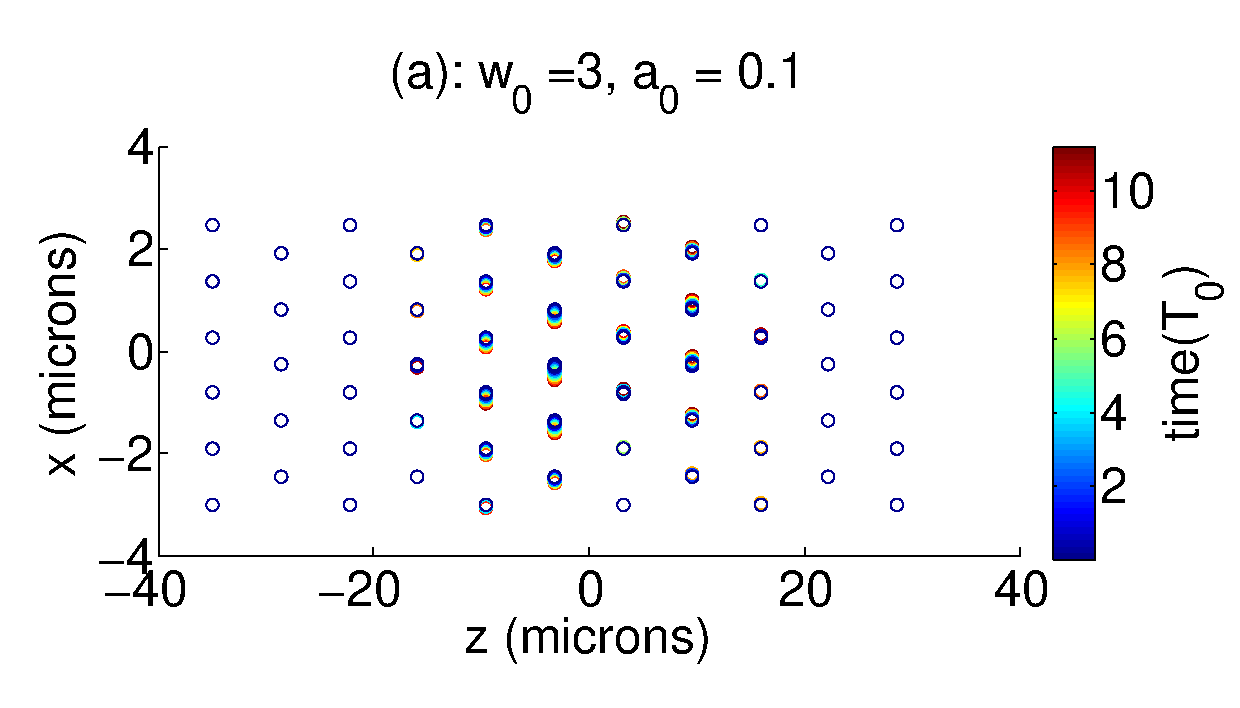
\includegraphics[width =8cm]{../chapitre2/images/a0_0p1w0_3.pdf}
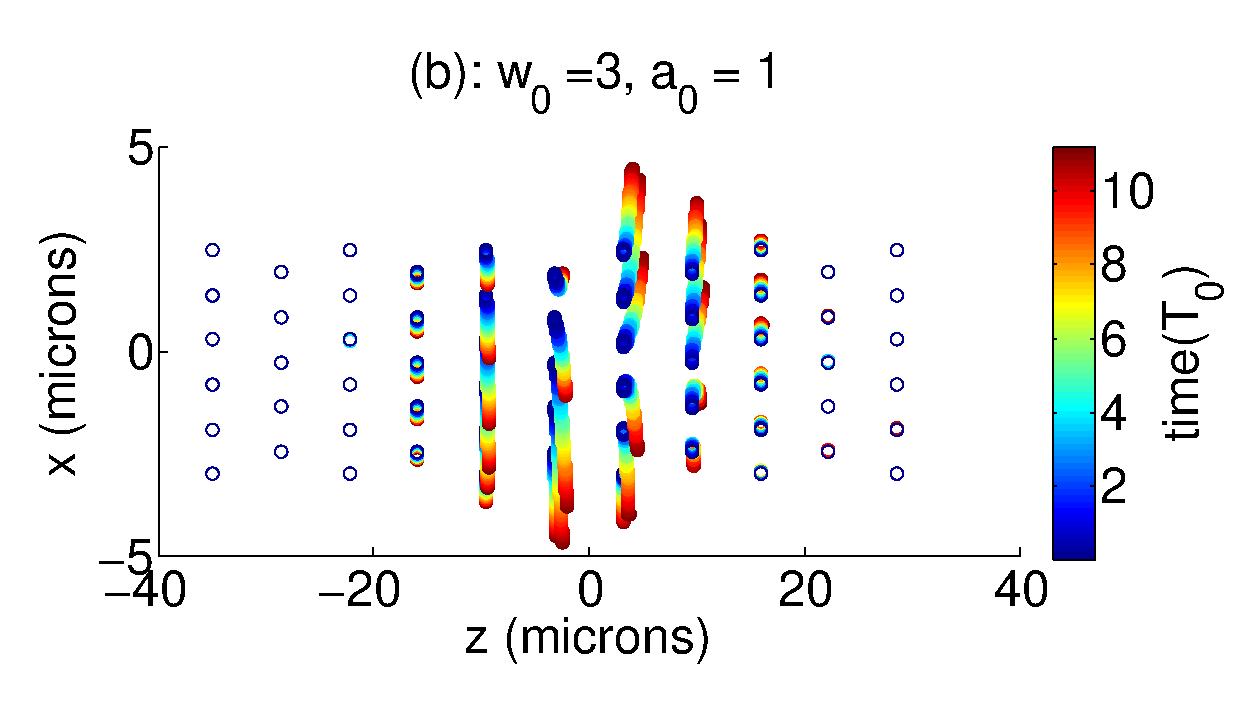
\includegraphics[width =8cm]{../chapitre2/images/a0_1w0_3.pdf}\\}
\makebox[\textwidth][c]{
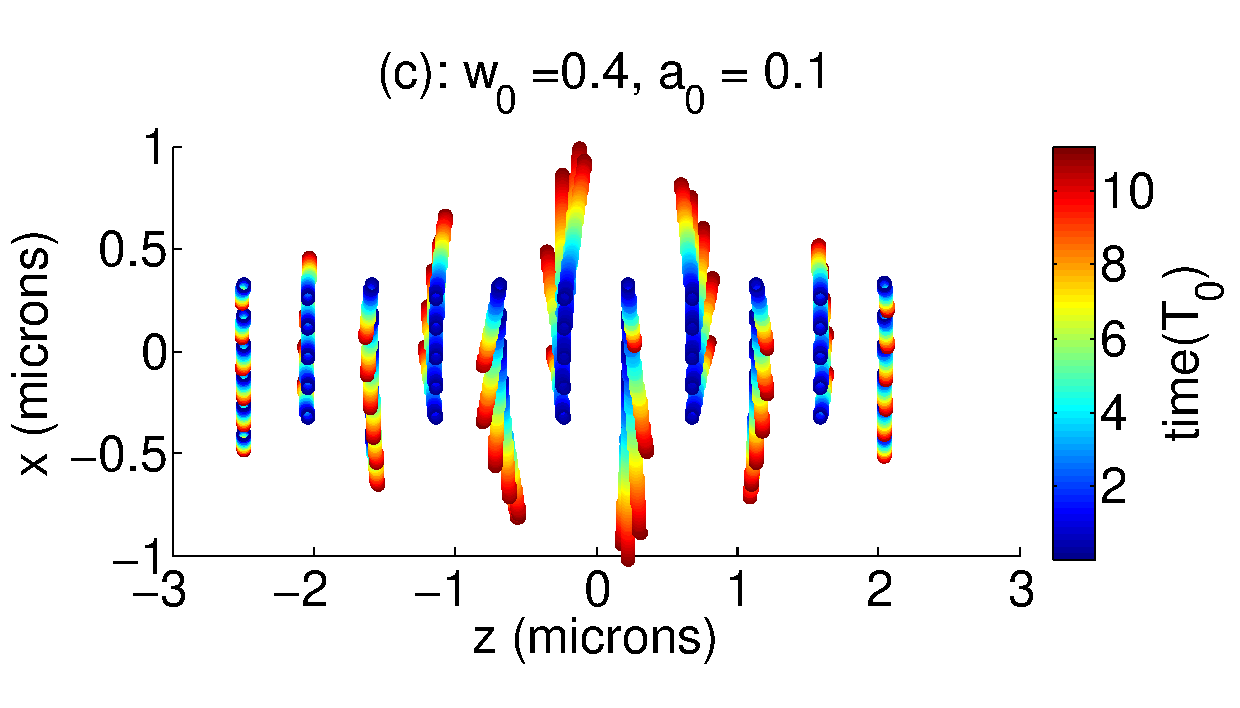
\includegraphics[width =8cm]{../chapitre2/images/a0_0p1w0_0p4.pdf}
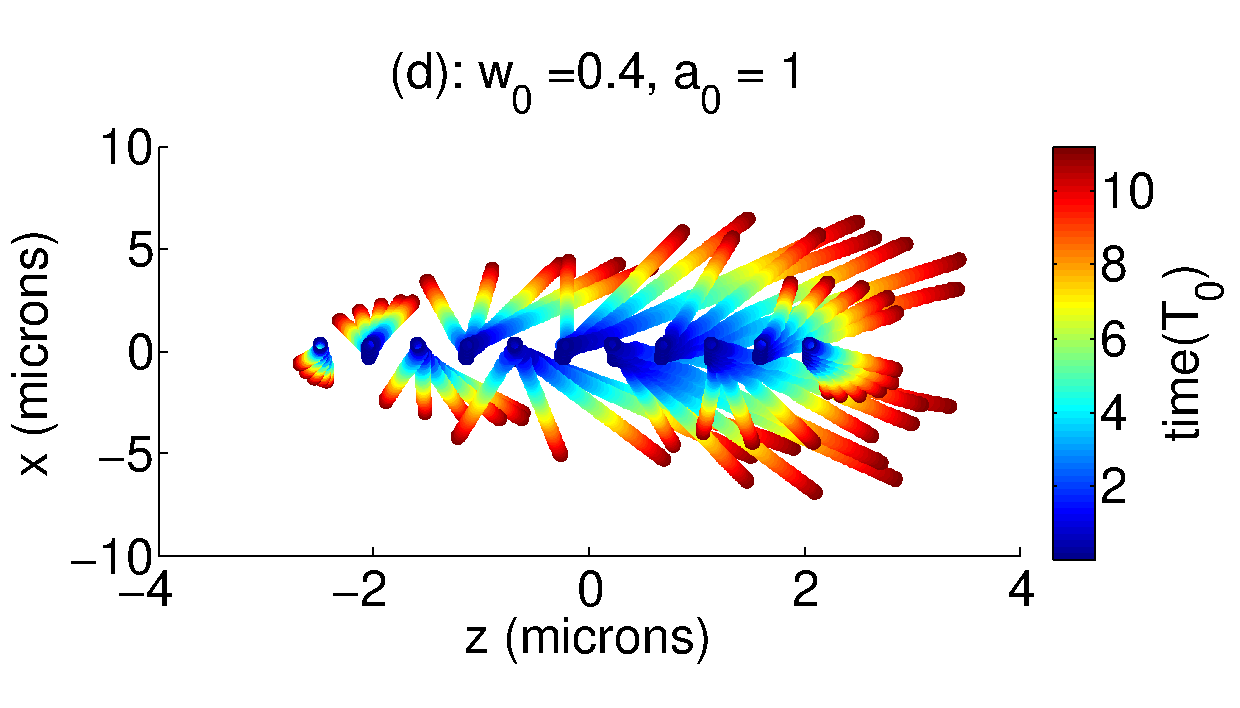
\includegraphics[width =8cm]{../chapitre2/images/a0_1w0_0p4.pdf}\\}
\caption{\label{fig:poneffect_sim}63 test electron trajectories in a Gaussian beam. All particles are injected at time $t=0$ when the laser is at focus. Particles are initially at rest and located in the domain $x_{i0}\in [-w_0 \ \ w_0]$, $z_{i0} \in [-Z_r \,Z_r]$. The laser is $30\,\mathrm {fs}$ FWHM and the simulation performed from $t=0$ to $t =30\,\mathrm{fs}$. Laser parameters:  (a) $w_0 = 3\,\mathrm{\mu m}$, $a_0 = 0.1$, (b) $w_0 = 3\,\mathrm{\mu m}$, $a_0 = 1$, (c) $ w_0 = 0.4\,\mathrm{\mu m}$, $a_0 = 0.1$, (d) $w_0 = 0.4\,\mathrm{\mu m}$, $a_0 = 1$,}
\end{figure}

\noindent  We now take test particles initially at rest in the plane $[x,z]$, where $x$ spreads along the laser waist, and $z$ along the Rayleigh length as described in Fig~\ref{fig:poneffect_sim}. At $t=0$, the test electron trajectories are calculated using a 3 dimensional code based on the field calculation presented in the following section~\ref{subsection:First orders field decomposition for strong laser focus}.  The final gained electron energies are given in Fig~\ref{fig:FinalElectronSpectra} and increase in a strong focusing geometry. 

\begin{figure}[H]
\begin{center}
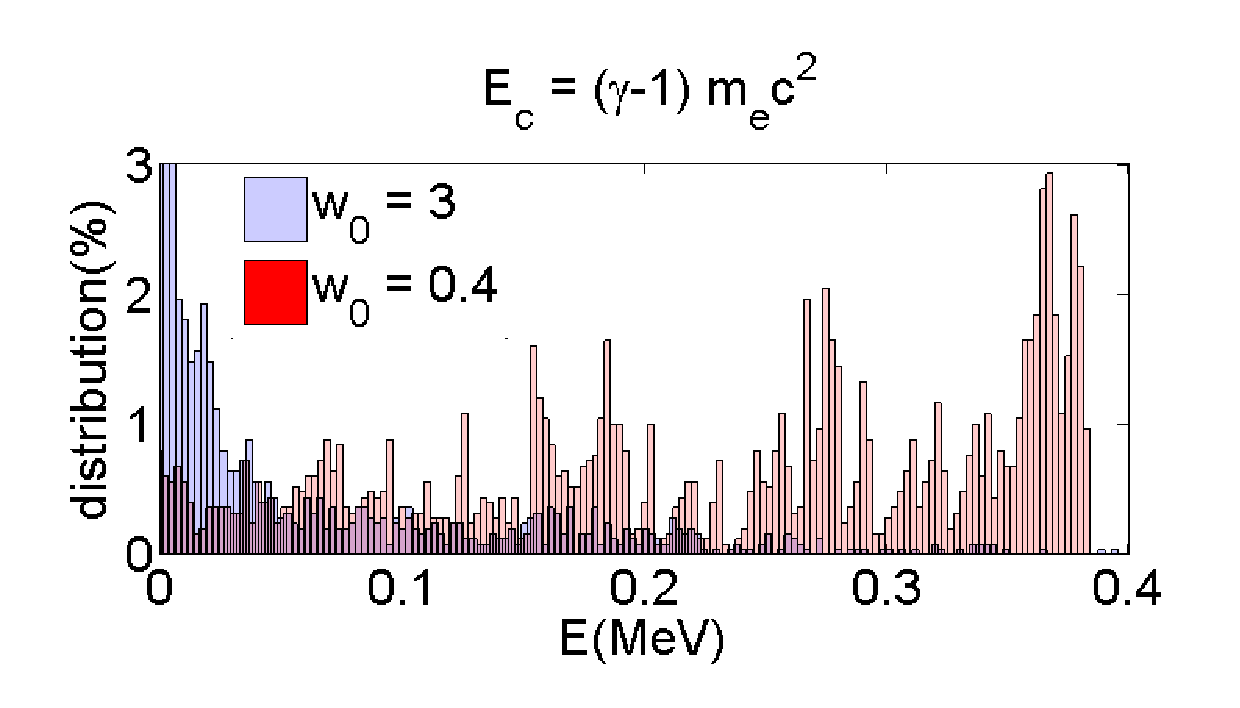
\includegraphics[width =0.8\textwidth]{../chapitre2/images/FinalEnergySpectra-comparaison.pdf}
\caption{\label{fig:FinalElectronSpectra}Final energy distribution after $t = 30\,\mathrm{fs}$ at $a_0 = 1$ for  $w_0 = 0.4$ (red) and $w_0 = 3$ (blue) for 2500 test particles}
\end{center}
\end{figure}

\noindent The results show enhanced acceleration in the case of strong focusing geometry, a direct consequence of the increasing ponderomotive potential in all directions (radial and longitudinal).

\subsection{Non-ponderomotive laser acceleration}\label{subsub:Non ponderomotive laser acceleration}


Here we wish to examine the other asymptotic case of an electron interacting with an electromagnetic field with no consideration for ponderomotive effects. 
This consists in integrating Eq~\ref{relativisticMotionEq0}, corresponding to the plane-wave approximation, and leads to the trivial result:



\begin{subequations}
\label{relativisticMotionEq0-int}
\begin{align}[left = \empheqlbrace\,]
&\gamma v_x - \frac{e}{m_e}A_x = \gamma_0 v_{x0} - \frac{e}{m_e}A_{x0}  \label{relativisticMotionEq0-1} \\
&\gamma v_y - \frac{e}{m_e}A_y = \gamma_0 v_{y0} - \frac{e}{m_e}A_{y0}  \label{relativisticMotionEq0-2} \\
&\gamma v_z -\frac{e}{m_e}A_z-\gamma c =\gamma_0 v_{z0}-\frac{e}{m_e}A_{z0} -\gamma_0 c  \label{relativisticMotionEq0-3} 
\end{align}
\end{subequations}

\noindent to which we add the relation:
\begin{equation}
\label{eq:Gamma-factor}
\gamma^2 = 1+\gamma^2\frac{v_x^2}{c^2}+\gamma^2\frac{v_z^2}{c^2}
\end{equation}

\noindent To simplify the resolution, the laser is polarized along $x$, such that $A_y = A_z =0$ at all time.
We define $a_0 = \frac{e}{m_e c}(A_{x0}-A_x) $ for better clarity.

\begin{subequations}
\label{relativisticMotionEq0-int}
\begin{align}[left = \empheqlbrace\,]
&\gamma v_x/c -\gamma_0 v_{x0}/c = a_0 \label{relativisticMotionEq0-1} \\
&\gamma (1 - v_z/c) =\gamma_0 (1 - v_{z0}/c ) \label{relativisticMotionEq0-3} 
\end{align}
\end{subequations}

\noindent The combination of Eq~\ref{relativisticMotionEq0-int} and relation~\ref{eq:Gamma-factor} gives:


%\begin{subequations}
%\begin{align}[left = \empheqlbrace\,]
%&\gamma^2 v_x^2/c^2 =(\gamma_0 v_{x0}/c + a_0)^2 \label{relativisticMotionEq0-1} \\
%&\gamma^2 (1 -v_z/c)^2 =\gamma_0^2(1 - v_{z0}/c )^2 \label{relativisticMotionEq0-3} 
%\end{align}
%\end{subequations}
%$$
%\gamma^2(1 - \frac{v_z^2}{c^2})= 1+\gamma^2\frac{v_x^2}{c^2}
%$$
%$$
%2\gamma^2 (1 -v_z/c) =\gamma_0^2(1 - v_{z0}/c )^2 + 1+ (\gamma_0 v_{x0}/c + a_0)^2
%$$
%$$
%(1 -v_z/c) = \frac{2\gamma_0^2(1 - v_{z0}/c )^2 }{\gamma_0^2(1 - v_{z0}/c )^2 + 1+ (\gamma_0 v_{x0}/c + a_0)^2}
%$$

\begin{equation}
(1 -v_z/c) = 2(1 + \frac{1+ (\gamma_0 v_{x0}/c + a_0)^2}{\gamma_0^2(1 - v_{z0}/c )^2})^{-1}
\end{equation}

\noindent and 

\begin{equation}
\gamma = \frac{\gamma_0}{2}(1 - v_{z0}/c )(1 + \frac{1+ (\gamma_0 v_{x0}/c + a_0(t))^2}{\gamma_0^2(1 - v_{z0}/c )^2})
\end{equation}


\noindent In this formulation, we see that an electron initially at rest can gain energy from the laser according to the scaling law:
%$$
%1-v_z/c = \frac{2}{2+a_0^2}
%$$

$$
(\gamma -1)m c^2 [\,\mathrm{MeV}]  \approx  \frac{a_0^2}{2} 
$$

\noindent Note that the laser will contribute to the electron acceleration when, by definition, $\gamma - \gamma_0 > 0$. The previous derivation shows that for some initial value of the vector potential $A_{x0}$, we can have $\gamma - \gamma_0 <0$, which corresponds to a deceleration of the electron by the laser.\\

%\begin{subequations}
%\begin{align}[left = \empheqlbrace\,]
%&\frac{e(A_{x0}-A_{xf}) }{m_e\gamma_0v_{x0}} \ge 0\\
%&\frac{e(A_{x0}-A_{xf})}{\gamma_0m_ev_{x0}} \le -2
%\end{align}
%\end{subequations}



\noindent We define the \g{dephasing length} as the distance the electron has to propagate in order to accumulate a phase difference of $\pi/2$ with the driving laser when propagating in the direction $z$, for a vector potential of the form $a(t) = a_0\cos (\omega_0t -k_0z)$.
For this scaling relation, we impose $u_{x0} = 0$ and $\beta_0 = v_{z0}/c$. 
 Indeed, the phase difference is:
$$
\phi(t) = \omega_0 t- k_0 z(t) 
$$
\noindent which implies 
$$
\phi(t)' = \omega_0(1 - \frac{v_z}{c}) = \omega_0\frac{\gamma_0}{\gamma}(1 - \frac{v_{z0}}{c}) 
$$

\noindent Using the relation $\phi'(t)z'(\phi) = z'(t)$ we find this dephasing length equals:
%
%\begin{equation}
%z'(\phi)= \frac{\gamma v_z}{\gamma_0\omega_0(1-v_{z0}/c)}=\frac{1}{2\omega_0}(  \frac{1+ (\gamma_0 v_{x0}/c + a_0(t))^2}{\gamma_0^2(1 - v_{z0}/c )^2} - 1)
%\end{equation}

\begin{equation}
Z_{deph} = \frac{\lambda_0}{4}\gamma_0^2(1+\beta_0)(\frac{a_0^2}{4}(1+\beta_0)+\beta_0)
\end{equation}

\noindent For an efficient acceleration effect of the laser, this value has to be greater than the Rayleigh length of the laser used to accelerate electrons. Of course, since what matters is the energy gain from the laser, when $\beta_0$ is close to one, the electron has a ballistic trajectory and hardly interacts with the laser such that when $Z_{depth}$ tends to infinity, $\gamma - \gamma_0$ tends to zero. In other words, for an efficient acceleration of the electron by the laser, there is an optimal $Z_{eff}>Z_R$ value allowing the electron to stay phase-locked to the laser and gain energy from the field.




\subsection{Strong focusing field decomposition}\label{subsection:First orders field decomposition for strong laser focus}

A monochromatic electromagnetic field propagating in vacuum can easily be propagated from one plane to another in the Fourier space (Fourier transformed relative to $(x,y)$ coordinates, then multiplication by a propagation transfer function). This is convenient for a polarized field since it can be considered "scalar". In real life however, an electromagnetic field has 6 degrees of freedom $(E_x,E_y,E_z,B_x,B_y,B_z)$. Naively, retrieving the full field from a plane requires using the scalar approach 6 times, one per degree of freedom. In reality, the real degree of freedom is reduced to 2 because of Maxwell's equations~\cite{pHdQuesnel}, which means for example that if both $E_x$ and $E_y$ are known, all other components (namely $E_z,B_x,B_y,B_z$) can be calculated without ambiguity. \\


\noindent If we consider a linearly polarized Gaussian beam $E_x$ propagating along $z$, its field does not satisfy the electromagnetic wave equation but instead the so-called Paraxial Equation. As a consequence, when one gets to the strong focused regime, that is to say when the paraxial approximation is no longer valid, only one component of the field $E_x$ is not enough to quantify the field in focus. In particular, suppose $E_x$ is a linearly polarized Gaussian beam along the direction $x$, and $E_y =0$ everywhere. Since $\nabla. E = \partial_xE_x +\partial_z E_z= 0$:

\begin{equation}\label{partial_derivation}
\begin{split}
\partial_z E_z(x,y,z) &=-\partial_x [\iint_{\mathbb{R}^2}E_x(k_x,k_y,z)e^{-ik_xx-ik_yy} dk_xdk_y] \\
 & =-\partial_x [\iint_{\mathbb{R}^2}E_x(k_x,k_y,0)e^{-iz\sqrt{k^2 - k_x^2-k_y^2}}e^{-ik_xx-ik_yy} dk_xdk_y] 
\end{split}
\end{equation}

\noindent Where the square root function is defined on complex number ($\sqrt{-1} = - i$ according to Eq~\ref{partial_derivation} convention). The integration of Eq~\ref{partial_derivation} in focus, which we define by $z=0$, shows that the $E_z$ component can not be equal to zero and is given by:


\begin{equation}\label{Ez_comp}
 E_z(x,y,z) = \iint_{\mathbb{R}^2}\frac{k_xe^{-iz\sqrt{k^2 - k_x^2-k_y^2}}}{\sqrt{k^2 - k_x^2-k_y^2}}E_x(k_x,k_y,0)e^{-ik_xx-ik_yy} dk_xdk_y
\end{equation}

\noindent where $E_x(k_x,k_y,0)$ is the Fourier transform of $E_x$ at focus.

\noindent The formula shows, as illustrated by Fig~\ref{fig:composanteEz} that for very small focal spot sizes relative to the laser wavelength, $E_z$ is no longer negligible relative to $E_x$, such that the polarization of the field has a component along $z$. Therefore, the force exerted by charged particles when the focal spot compares with the laser wavelength has to be calculated using these components of the field. We will see this can have drastic consequences on the predicted result.

\begin{figure}[!h]
\centering
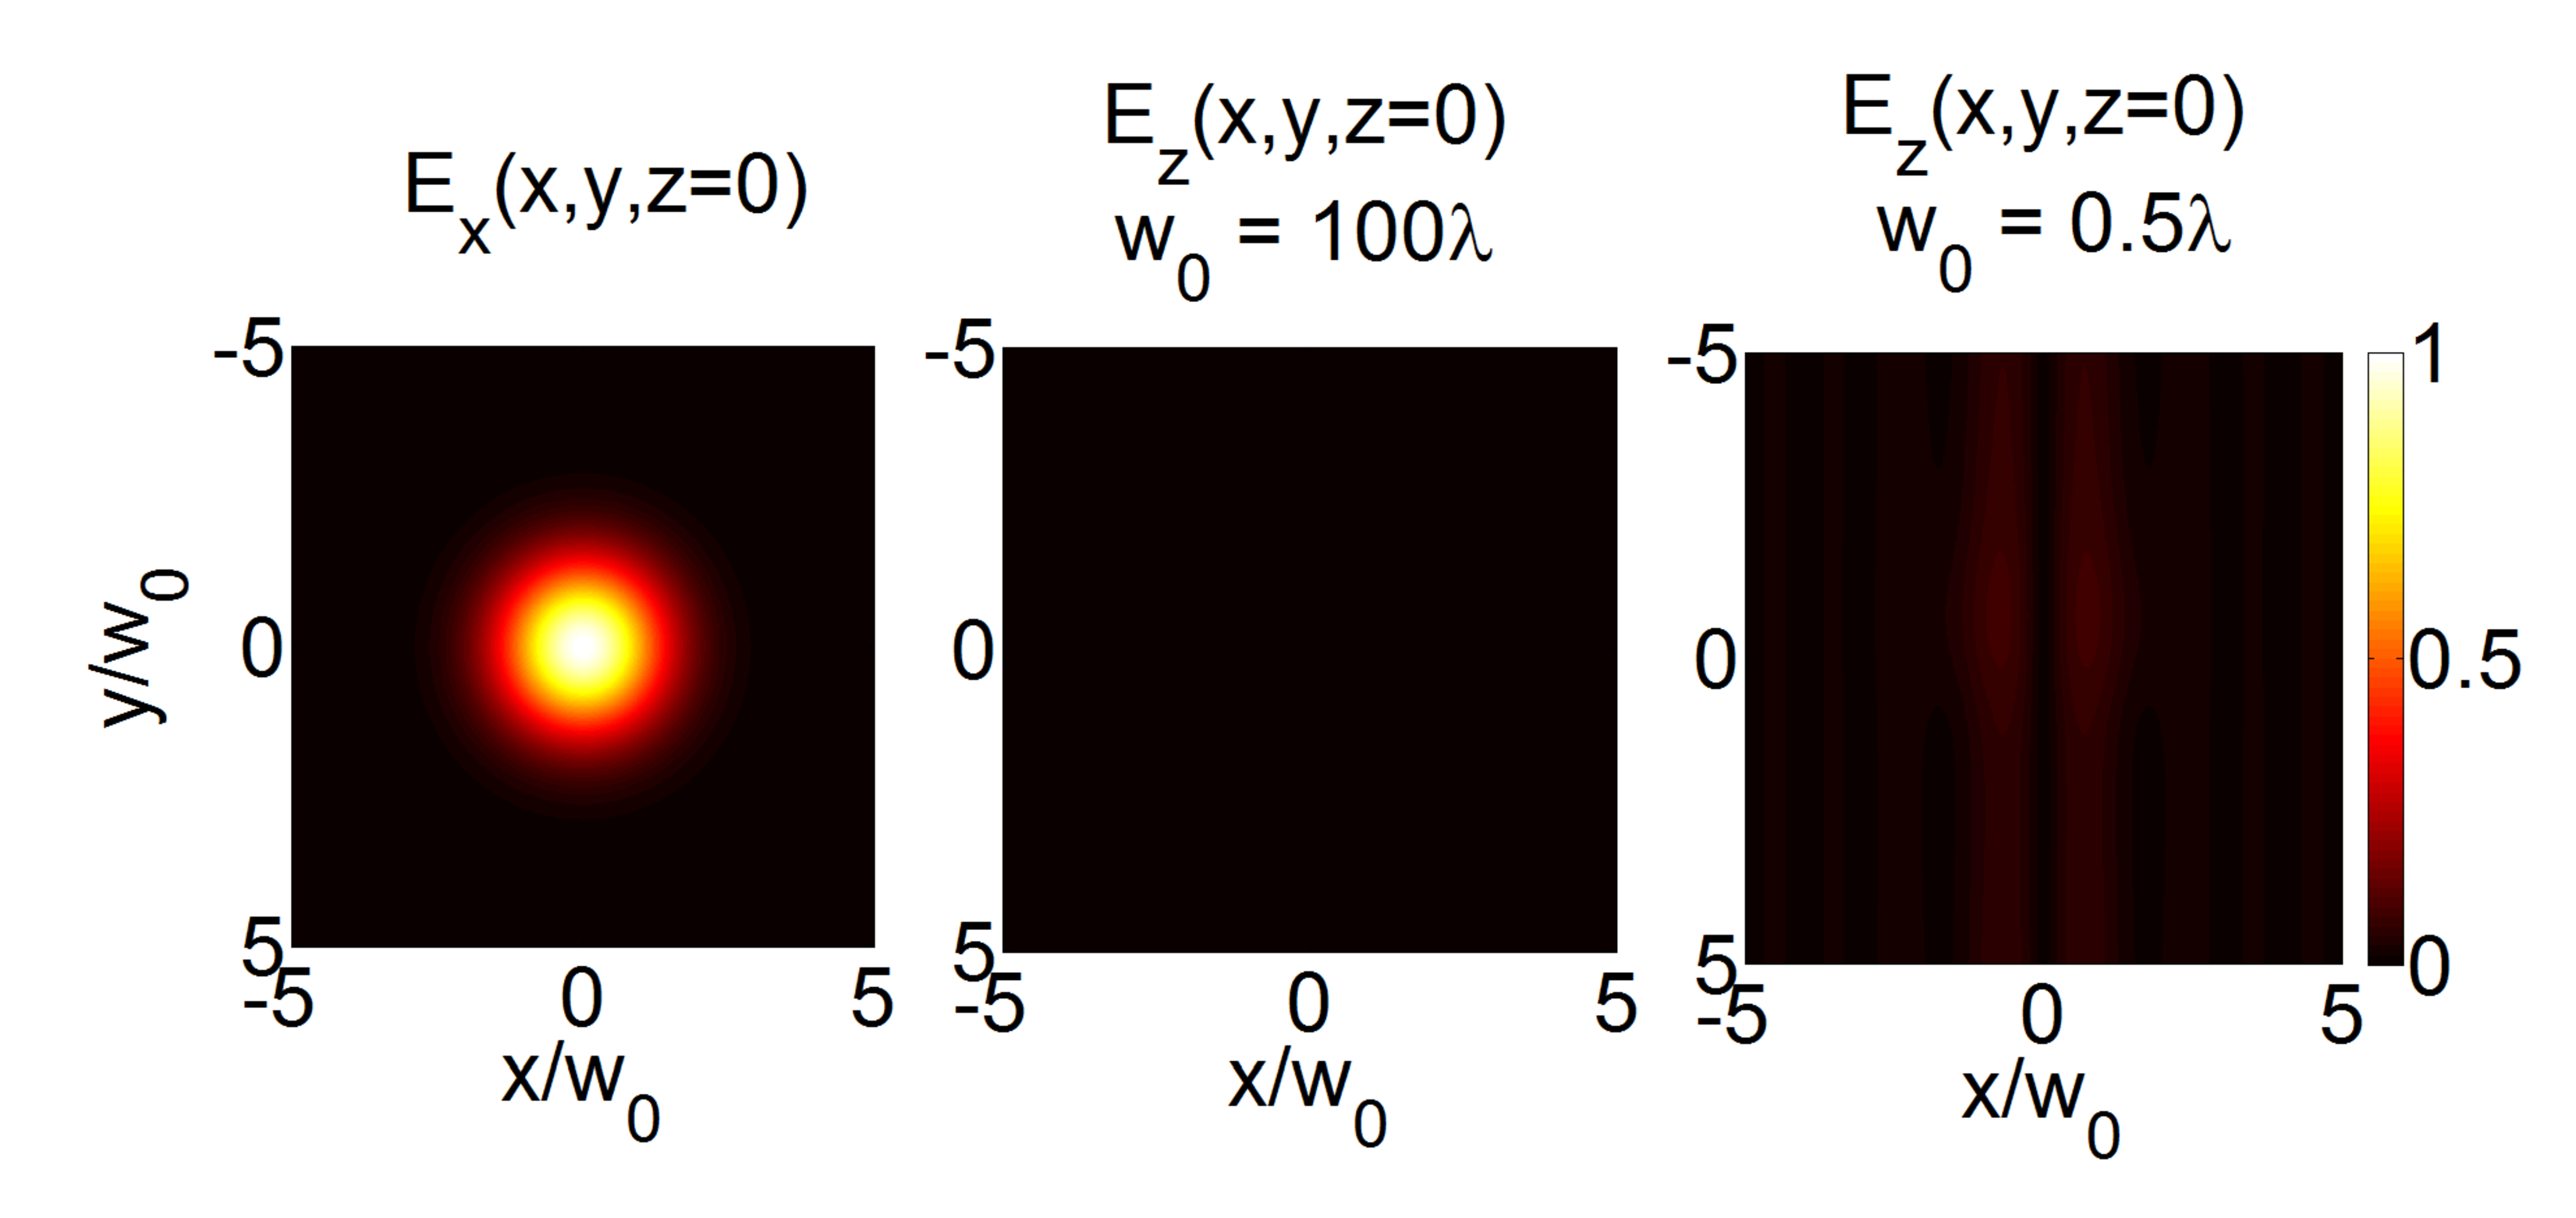
\includegraphics[width =12cm]{../chapitre2/images/composanteEz.pdf}\\
\caption{\label{fig:composanteEz} $E_x(x,y,z=0)$ is a Gaussian beam of waist $w_0$.  $E_z(x,y)$ calculated with Eq~\ref{Ez_comp} for $w_0 = 100\lambda$ and $w_0 = 0.5\lambda$ All images are normalized by the maximum value of $|E_x|$.}
\end{figure}

\noindent Since we want an analytical expression of the laser beam in order to calculate the trajectories of test electrons, we will rely on strong field decomposition. Indeed, it  has been shown \cite{quesnel1998theory} that the field can be developed relative to a small parameter $\epsilon = \frac{\lambda}{2\pi w_0}$


\begin{subequations}
\label{ex:expansionSeries}
\begin{align}[left = \empheqlbrace\,]
&E_x =\textcolor{red}{E_x^{(0)}} + \epsilon^2 E_x^{(2)} + ...\\
&E_y= \epsilon^2 E_y^{(2)} +... \\
&E_z = \epsilon E_z^{(1)} + \epsilon^3 E_z^{(3)}+...\\
&B_x=\epsilon^2 B_x^{(2)} \\
&B_y= \textcolor{red}{B_y^{(0)}} + \epsilon^2 B_y^{(2)}\\
&B_z=\epsilon B_z^{(1)} + \epsilon^3 B_z^{(3)}
\end{align}
\end{subequations}

\noindent where \textcolor{red}{the zeroth order} is the well-known Gaussian beam:

\begin{equation}
E_x^{(0)} = cB_y^{(0)} = \frac{E_0}{w(z)}e^{-ikz}e^{-ik\frac{r^2}{2q(z)}}e^{i\xi(z)}
\end{equation}

\noindent The higher order terms are calculated by identifying the terms of a polynomial series (we will not get into the details of the demonstration as it is very well described in \cite{quesnel1998theory}). Now artificially imposing a Gaussian envelope for the temporal profile (the field is no longer monochromatic) for $(x,y,z,t)$:



\begin{equation}
E_x^{(0)}  = \frac{w_0 E_0}{w(z)}\exp (-\frac{(t-z/c)^2}{t_0^2})\exp (-\frac{r^2}{w(z)^2})\cos(\xi(z) +\omega t - k z - k\frac{r^2}{2R(z)}+\phi_0)
\end{equation}

The series is expanded using~\ref{ex:expansionSeries} and gives us an accurate decomposition of the field at focus. We use this decomposition to calculate the trajectories of test electrons. This will be referred to later as our "3D particle code". We give in Fig~\ref{fig:shemaLaser} a schematic view of the system coordinates defined inside the particle code and used in hereafter.

%\noindent Where the waist is located at $z=0$.


\begin{figure}[H]
\begin{center}
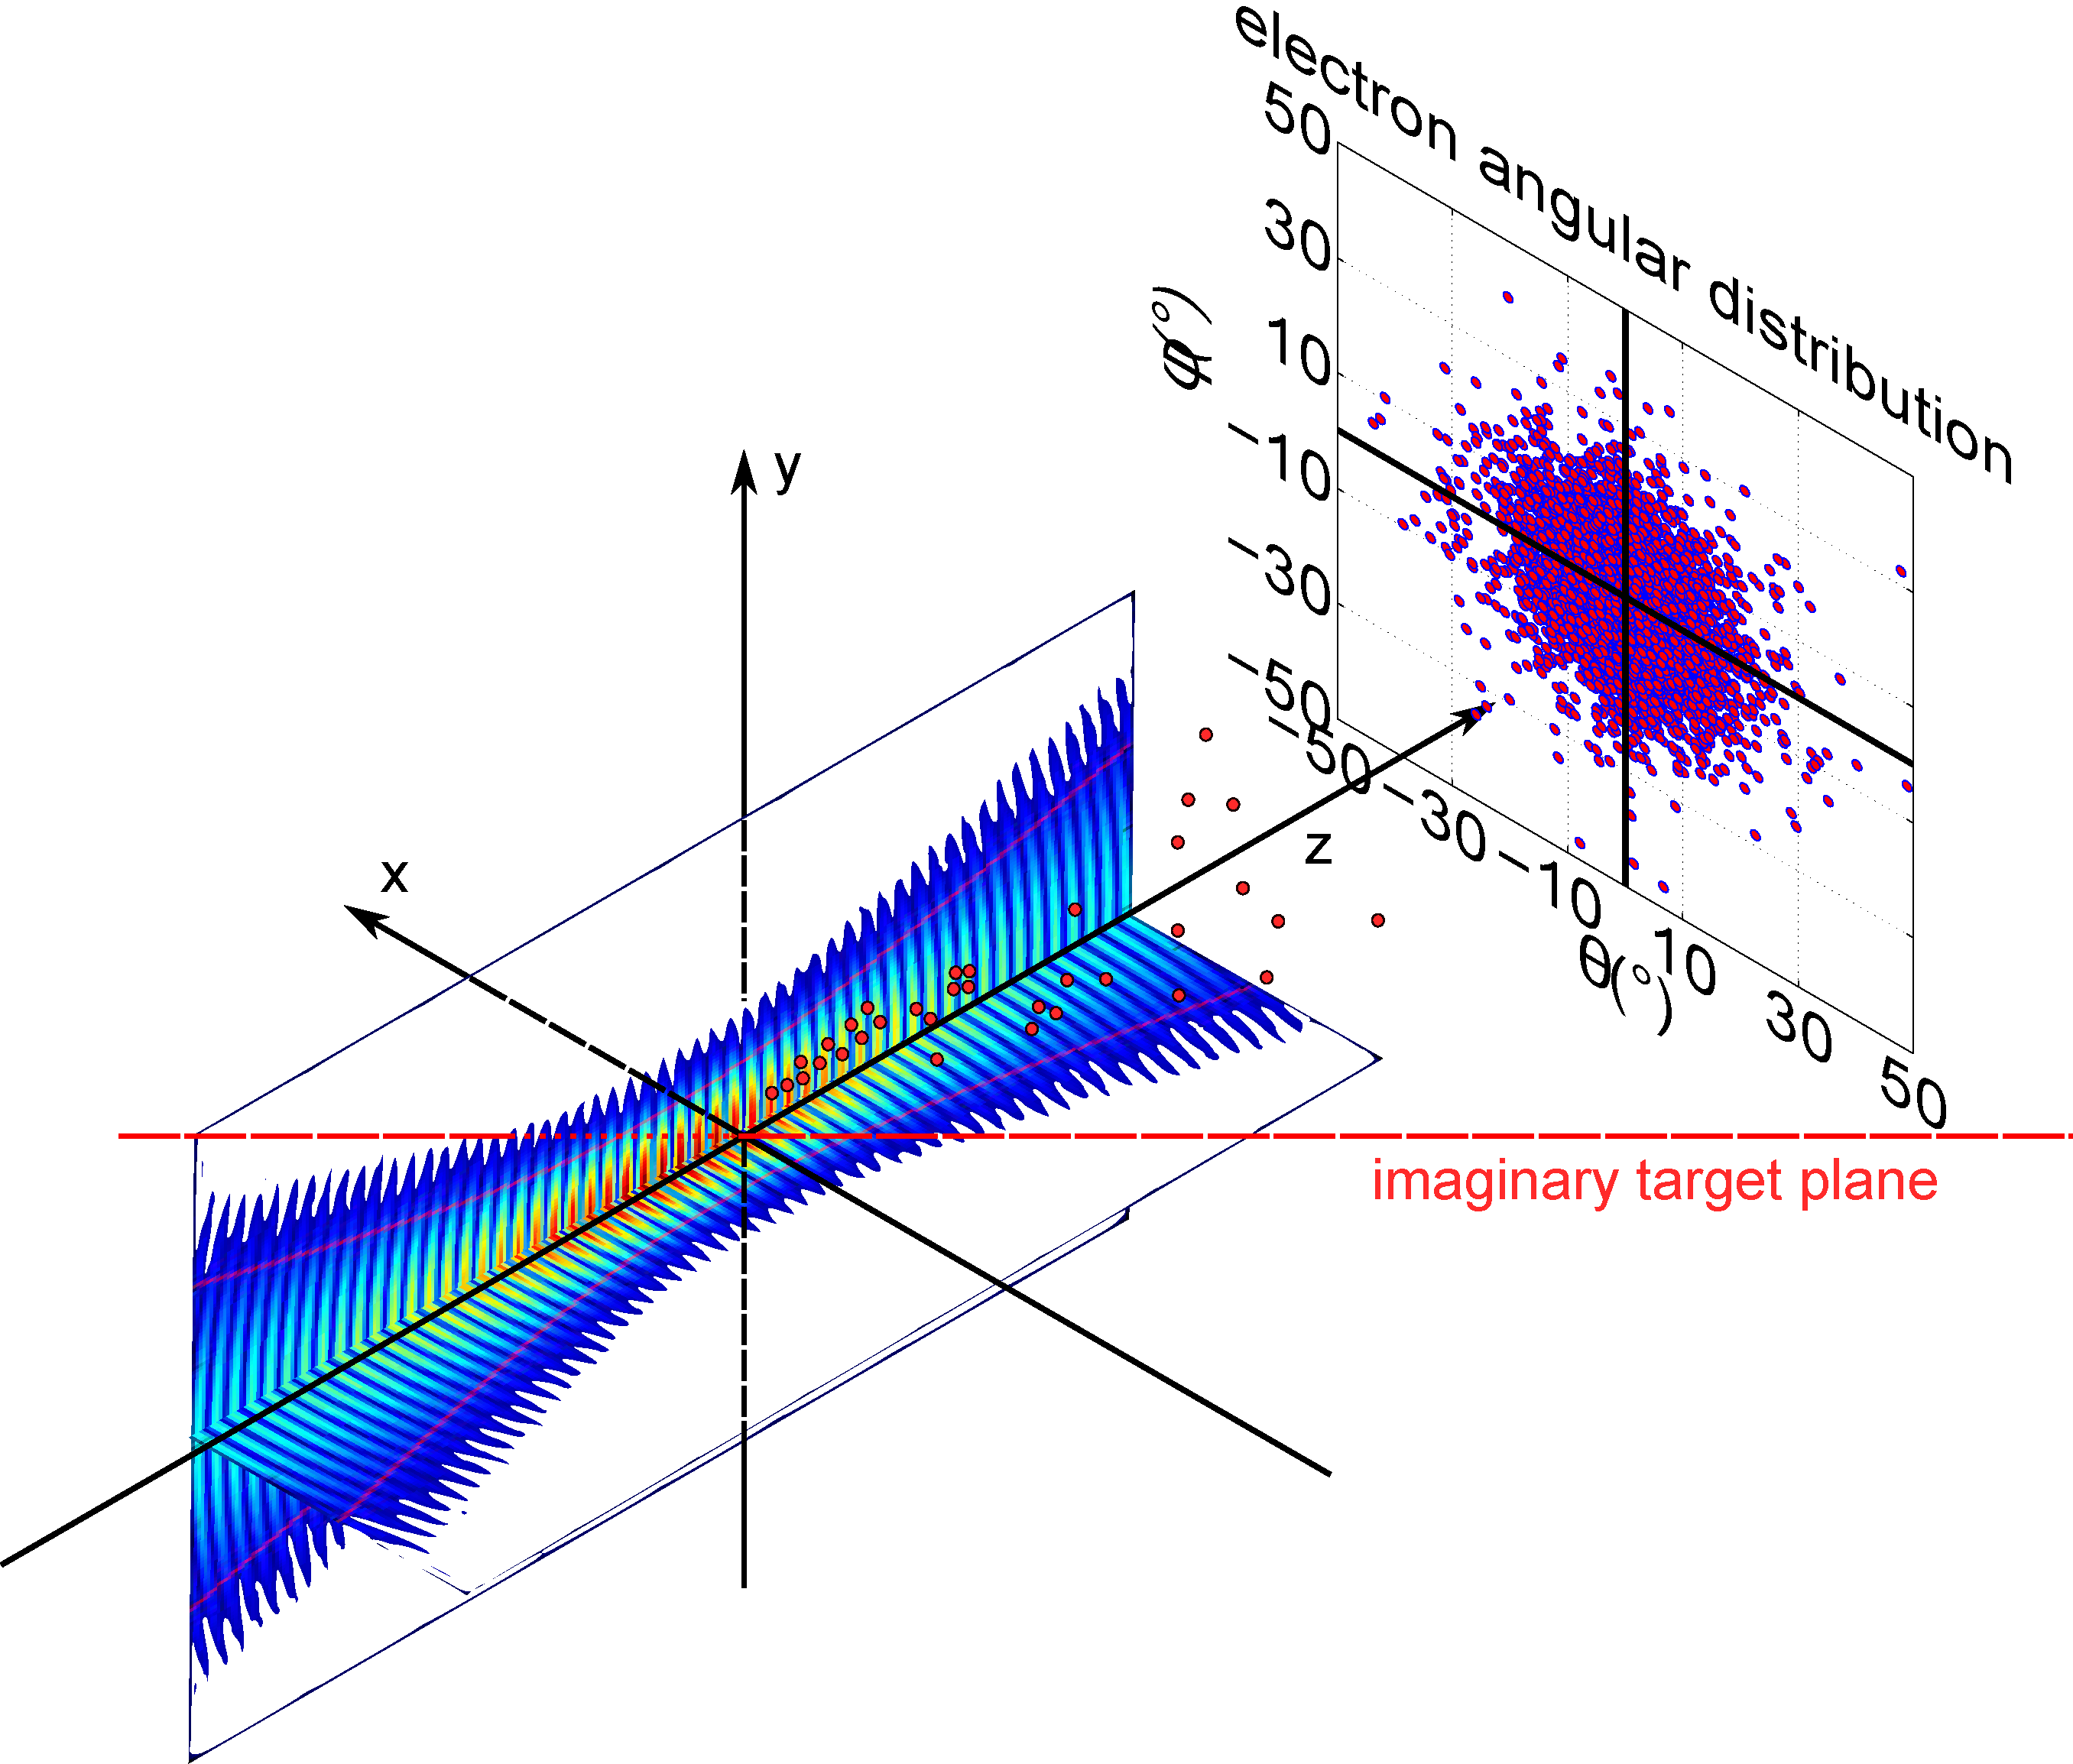
\includegraphics[width =\textwidth]{../chapitre2/images/shemaLaser.pdf}
\caption{\label{fig:shemaLaser}Schematic view of the 3D particle code: z is the direction of propagation and $x$ the direction of the zero order Gaussian beam $E_x^{(0)}$. $\theta$: angle in the (x,z) plane with the conventions $\theta<0$ toward the target normal, and $\phi$ the angle in vertical plane}
\end{center}
\end{figure}




%\noindent The field decomposition performed on ~\ref{fig:first-order-decomposition} gives a similar result than what we found with the Fourier~\ref{Ez_comp} decomposition: the field in focus undergoes a strong dependance in $z$, nearly 3 orders of magnitude greater for $w_0 = 0.5\lambda$ than for $w_0 = 100\lambda$.


\section{Hole formation and spectral shaping in vacuum}




\subsection{Two regimes of acceleration}\label{Two acceleration regime confirmation with 3D particle code}

We saw in Section~\ref{subsec:Relativistic ponderomotive force derivation} the role played by the ponderomotive force: a focused laser will expel electrons from the zone of highest intensity toward zones of lower intensity. The expression of the ponderomotive force indicates a radial force $\propto \nabla I$ independent of laser polarization. However, we also discussed the possibility for non-ponderomotive acceleration to occur when an electron escapes the laser field before we can consider an averaged, i.e. purely ponderomotive, acceleration. Taking again the example given in Section~\ref{subsec:Relativistic ponderomotive force derivation} of a $30\,\mathrm{fs}$, $a_0 = 1$ laser field, for the two cases $w_0 = 3\,\mathrm{\mu m}$ and $w_0 = 0.4$, we inject test particles initially at rest at time $t_{in} = 0$ (at that time, the laser is exactly at focus) and retrieve the angular emission profile of electrons with positive final momentum with respect to the direction of propagation. The result is given in Fig~\ref{Fig:EffetPondero_figurea0=1_a0=3}: on the left panel representing the final angular profile of the accelerated electrons, 2 populations are clearly visible namely (i) electrons radially spread by the purely ponderomotive effect, also corresponding to the lowest part of the spectrum ($\le 0.15\,\mathrm{MeV}$) and (ii) electrons accelerated in the direction of polarization of the laser forming two zones of higher energy ($>0.15 \,\mathrm{MeV}$). Depending on their initial position (i.e. phase) in the driving laser, electrons could be trapped in phase with the propagating laser such that they do not average over the whole acceleration path. This leads to the two distribution bulbs located on the polarization plane $\phi = 0^{\circ}$.

\begin{figure}[H]
\begin{center}
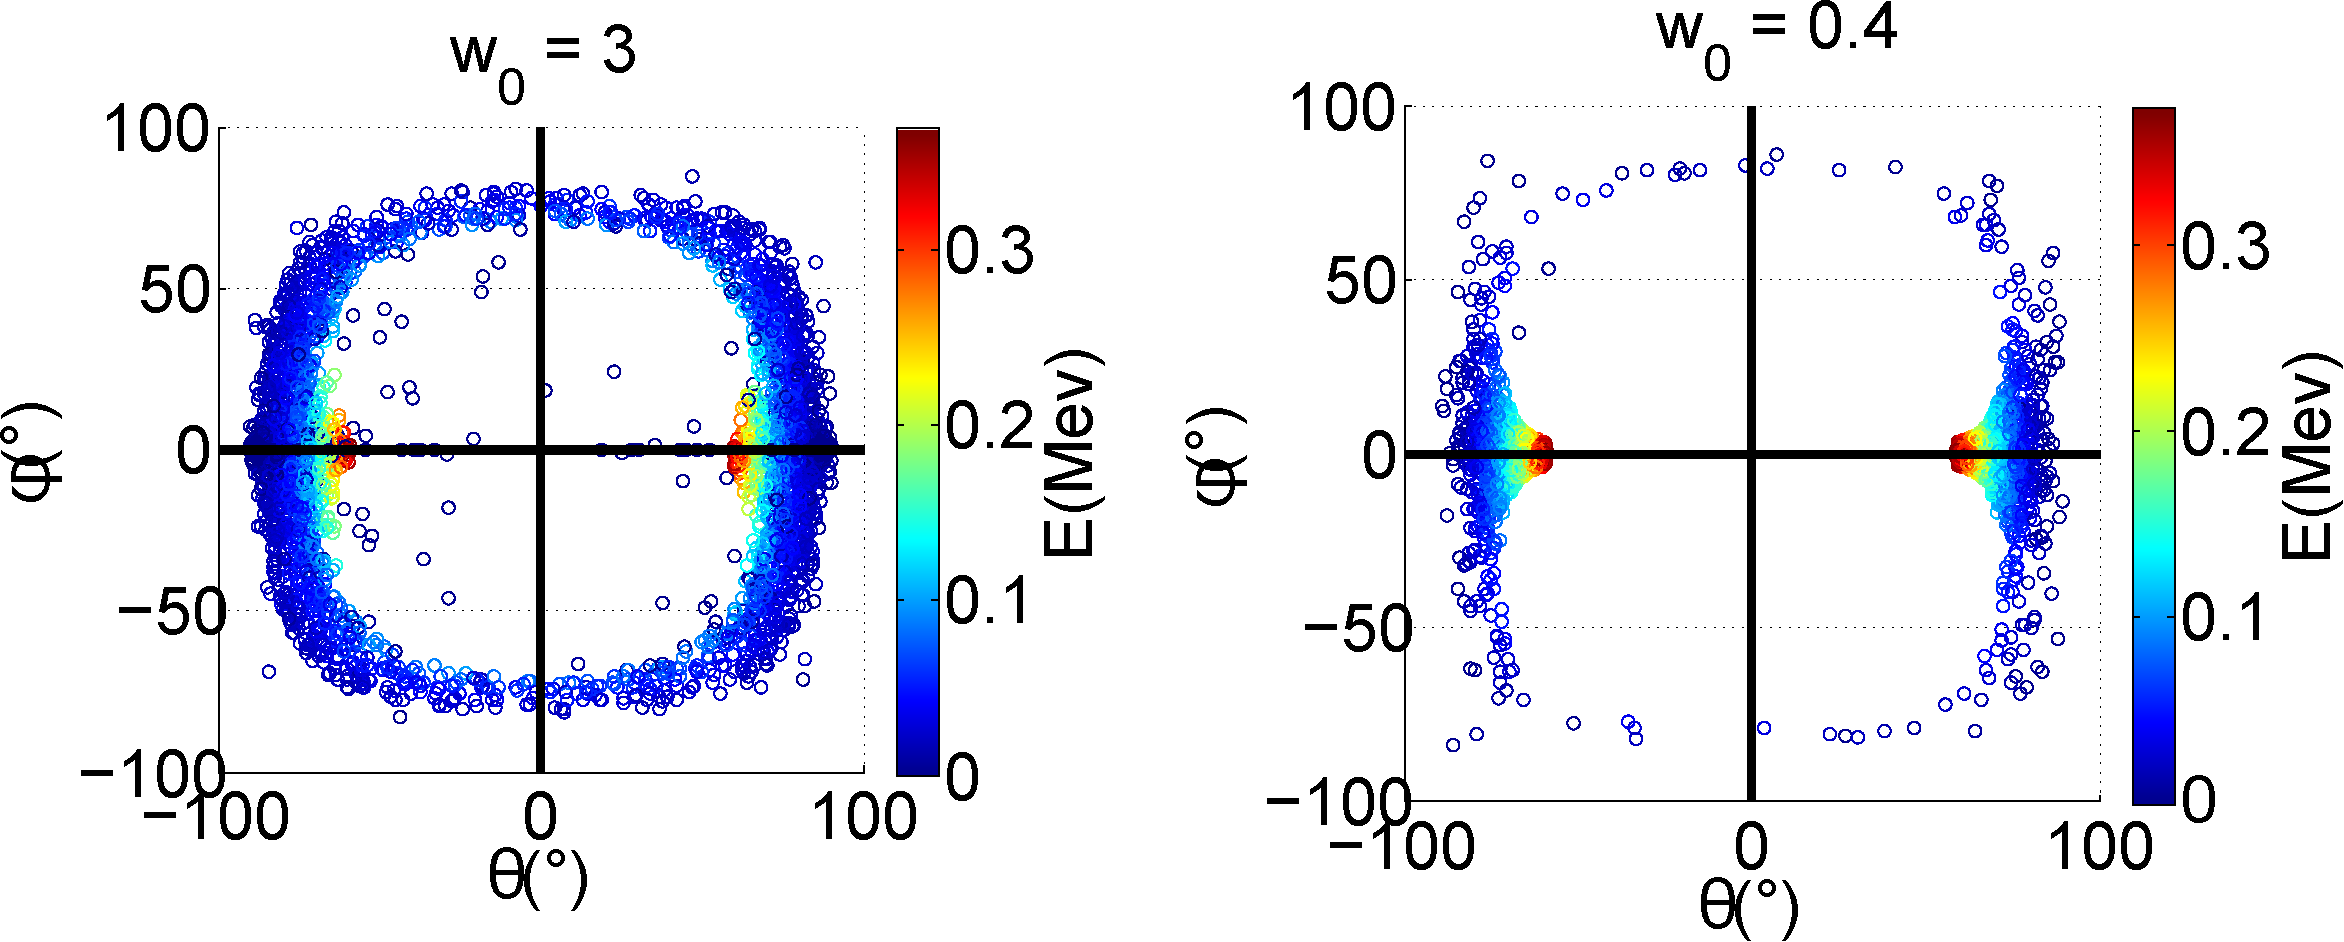
\includegraphics[width =\textwidth]{../chapitre2/images/EffetPondero_figurea0=1_w0=3_vs_w0=0p4fig.pdf}
\caption{\label{Fig:EffetPondero_figurea0=1_a0=3}Result of 3D particle code showing final electron angular distribution with final kinetic energy $E_c = (\gamma-1)m_ec^2$ in color scale. 5041 test particles initially at rest are randomly injected in the cylinder defined by $z_0 \in [-Z_R \ \ Z_R]$, $r_0\in [0 \ \ w_0]$ in a $\tau_{fwhm} = 30\,\mathrm{fs}$, $a_0 = 1$ focused laser beam polarized in the plane $\phi = 0$ with a waist of respectively $w_0=3$ (left) and $w_0 =0.4$ (right).}
\end{center}
\end{figure}

This non-ponderomotive electron acceleration by the laser was demonstrated experimentally in the relativistic case ($a_0 > 1$)~\cite{thevenet2015} as described in the following. Since the acceleration efficiency depends on the phase of injection, this mechanism is designated as "vacuum injection".\\


\subsection{Application to the relativistic case}

In a solid target experiment conducted on UHI100 at CEA~\cite{thevenet2015}, for a laser intensity $a_0 = 2.5$ and $w_0 = 5\,\mathrm{\mu m}$, non-ponderomotive acceleration (or vacuum injection) of electrons has been demonstrated. The electrons energies reached $\sim 10\,\mathrm{MeV}$ and were emitted in a collimated beam near the ponderomotive hole formed by the laser in the angular emission profile.\\

In~\ref{subsub:Non ponderomotive laser acceleration}, we defined a scaling length $Z_{eff}$ which, if greater than the laser waist, indicates that non-ponderomotive acceleration is dominant. Using the laser characteristics from CEA, we plotted $Z_{eff}$ in Fig~\ref{fig:Dephase_relativistic}.

\begin{figure}[H]
\begin{center}
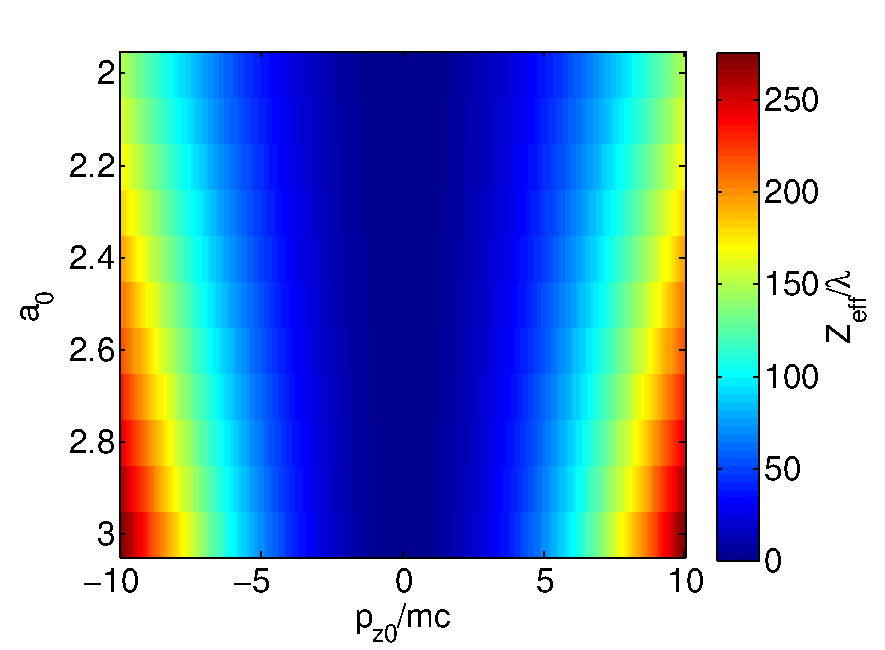
\includegraphics[width =0.6\textwidth]{../chapitre2/images/Dephase_relativistic.pdf}
\end{center}
\caption{\label{fig:Dephase_relativistic} $Z_{eff}$ as a function of $a_0$ and initial momentum $p_{z0}/mc$ from Fig~\ref{fig:Relativist3DpatCode_noInterferences} for relativistic case $a_0 \sim 2.5$. Here, $\lambda = 0.8\,\mathrm{\mu m}$}
\end{figure}


\noindent As described in~\cite{thevenet2015}, the experimental angular profile and emission spectra were reproducible combining 1D PIC simulations with a 3D particle code. The 3D particle code allowed one to calculate the electron trajectories once they have escaped the influence of the plasma. The PIC simulations are necessary to extract the "initial conditions", that is to say their initial momentum distribution and phase inside the laser. As a result of PIC simulations, the initial phase of electrons corresponds to a switch of the magnetic field from negative to positive values. 
In addition, the initial momentum distribution represented in Fig~\ref{fig:Relativist3DpatCode_noInterferences} was retrieved from 1D PIC simulations by probing the current of ejected particles at the position $n(x) = n_c/5$ (beginning of the plasma, the density in the simulation cell is imposed rigorously equal to zero above this limit). Using the 3D code presented previously, we reproduced the final angular emission of the electrons shown in Fig~\ref{fig:Relativist3DpatCode_noInterferences} using 5041 test electrons as already performed in~\cite{thevenet2015}. The final angular distribution showing a peak of energetic electrons located near the hole, and visible on Fig~\ref{fig:Relativist3DpatCode_noInterferences}, is exactly the profile measured in the experiment~\cite{thevenet2015}, which proves the consistency of the scaling parameter $Z_{eff}$ plotted in~\ref{fig:Dephase_relativistic}.



\begin{figure}[H]
\begin{center}
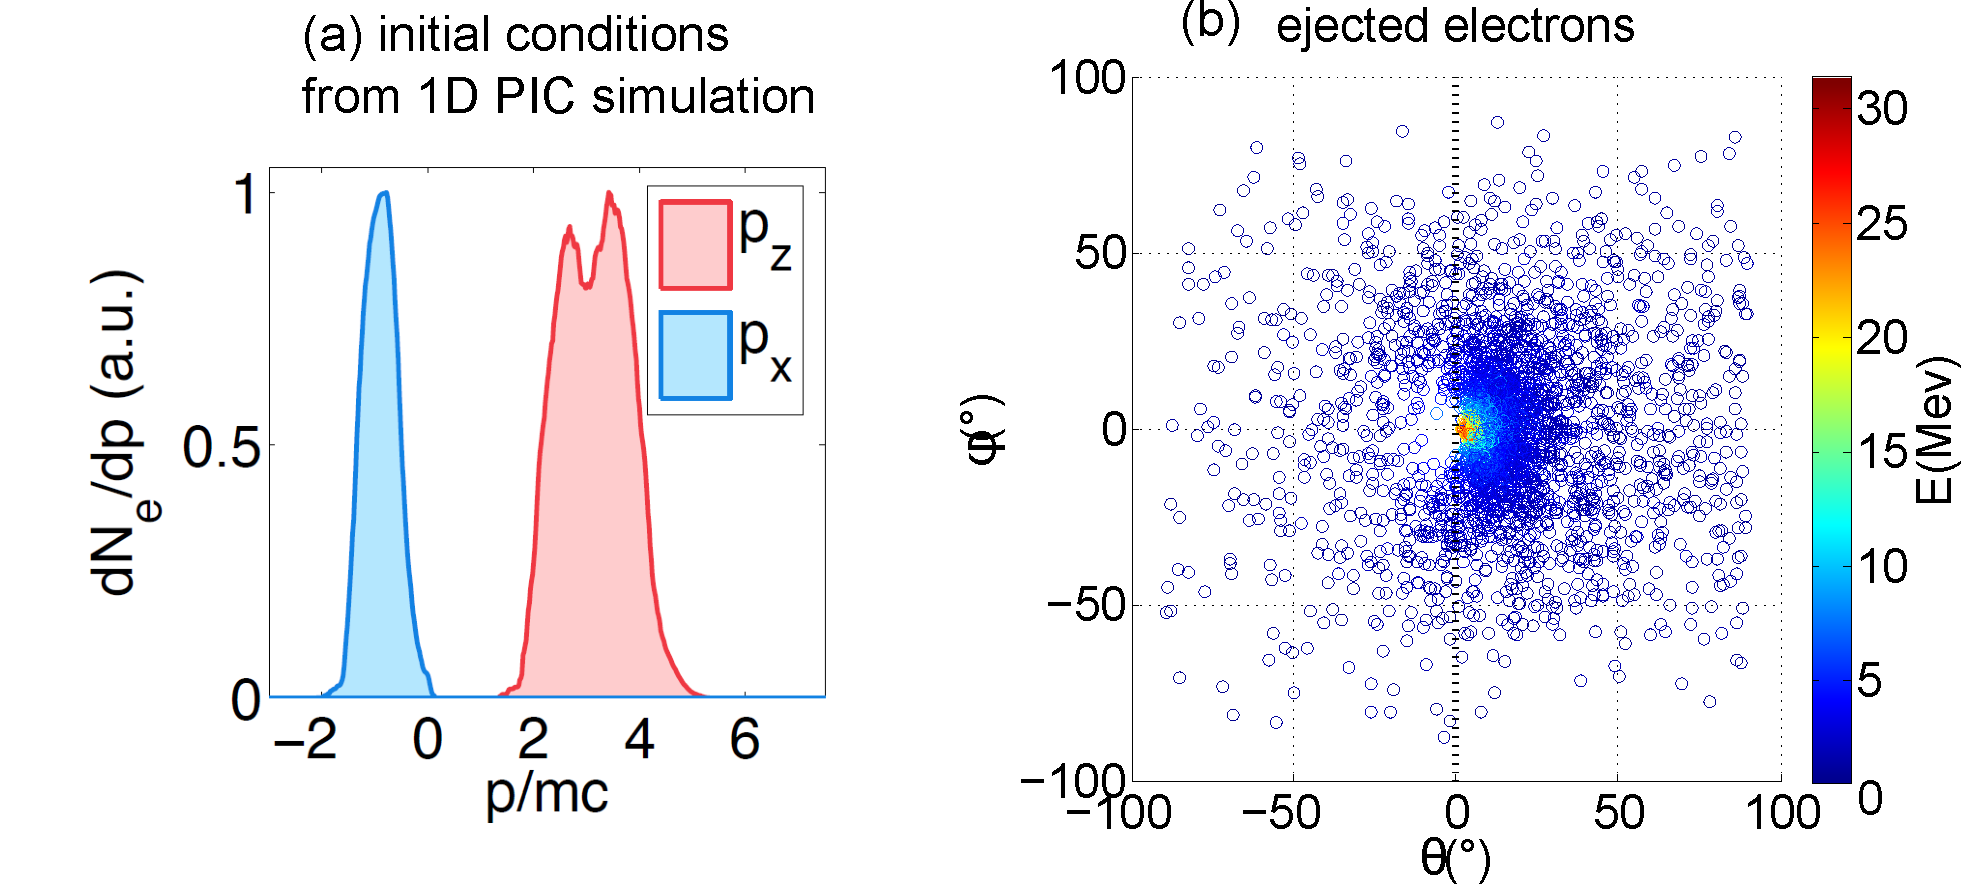
\includegraphics[width =0.9\textwidth]{../chapitre2/images/Relativist3DpatCode_noInterferences.pdf}
\end{center}
\caption{\label{fig:Relativist3DpatCode_noInterferences} (a) Initial conditions of injected electrons (screen shot from Reference~\cite{thevenet2015}) extracted from 1D PIC simulation. Particles are injected when the magnetic field $B_y$ switches to positive values with random distribution $t_0\in [-0.33\,\mathrm{fs} \ ;\ 0.33\,\mathrm{fs}] $ Laser conditions: $a_0 = 2.5$, $\tau_{FWHM} = 15\,\mathrm{fs}$, $w_0 = 5\mu m$ and $\lambda = 0.8\,\mathrm{\mu m}$. (b) Angular distribution of ejected electrons were (each point corresponds to an electron). The colorbar indicates the final energy in MeV.}
\end{figure}
%


%According to PIC simulations, electron which escape the plasma are injected when the magnetic field changes signs, periodically with the driving laser. We consider electrons to be ejected when they reach a distance $>0.5\lambda$ from the beginning of the plasma. By following only this "ejected" electrons over time, we can record the current through the position $x_0 = x_{end} - 0.1\lambda$.




\subsection{Application to the sub-relativistic case}

Based on the previous discussion, we can legitimately wonder whether vacuum injection is still efficient at sub-relativistic intensities.
We reproduce the previous analysis for $a_0 \sim 0.4$. At first sight, the problem looks similar and we expect to reproduce the experimental profile of ejected electrons shown in section~\ref{subsub:Spatial distribution of ejected electrons}. However, using our laser parameters, we find that the coherent length $Z_{eff}$ is smaller than the laser waist $w_0\sim 1.2-1.6 \lambda$. This means that the initial injection phase inside the laser will quickly depend on the probing plane using the PIC simulation, which makes it more difficult to clearly define. In Fig~\ref{fig:ConditionsInitiales-CWE} we give an example of what we can extract for 1D PIC simulation for $L = \lambda/10$, $a_0 = 0.4$ when placing a probe at position $0.1\lambda$ from the end of the plasma in vacuum. 
%We will impose the following injection conditions: 
%$t_0+\sin\theta x_0/c$

\begin{figure}[H]
\begin{center}
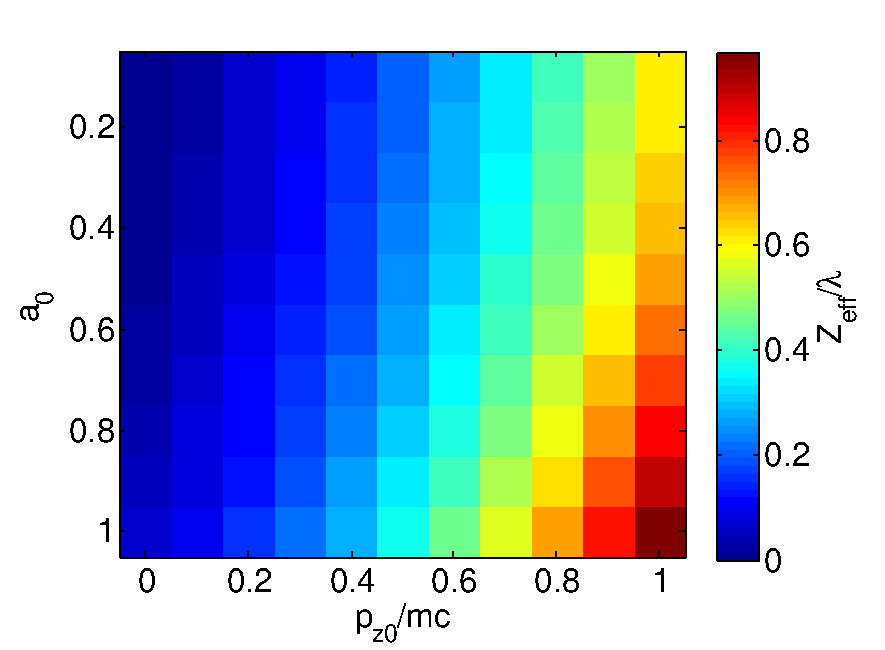
\includegraphics[width =0.6\textwidth]{../chapitre2/images/Dephase_nonrelativistic.pdf}
\end{center}
\caption{\label{fig:Dephase_nonrelativistic} $Z_{eff}$ as a function of $a_0$ and initial momentum $p_{z0}/mc$}
\end{figure}


\begin{figure}[H]
\begin{center}
\makebox[\textwidth][c]{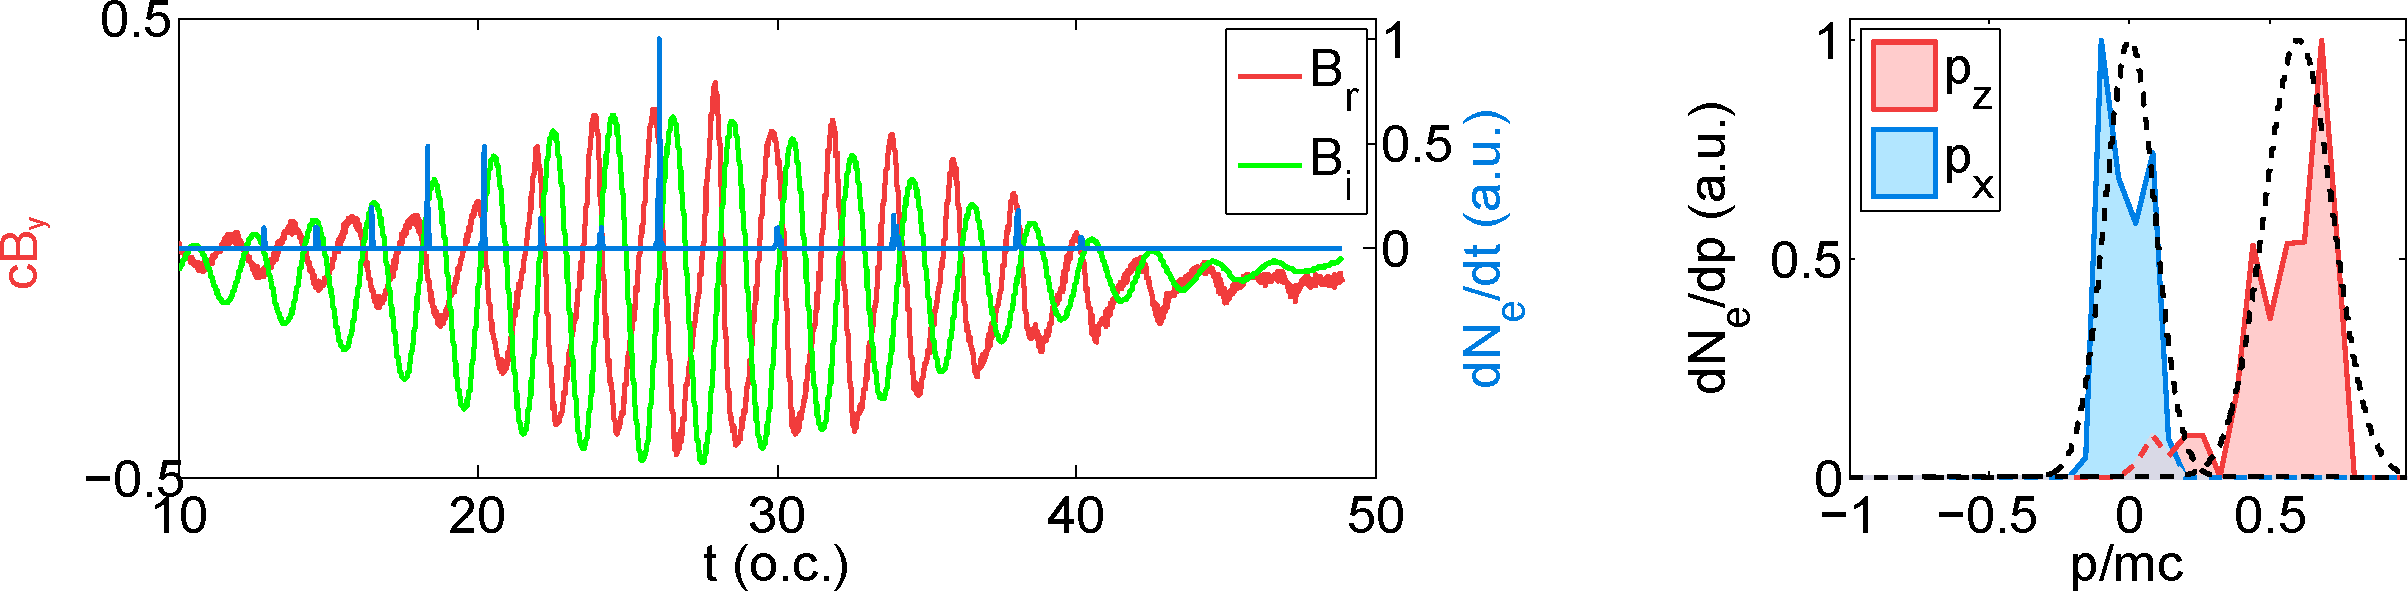
\includegraphics[width =17cm]{../chapitre2/images/ConditionInitiales-CWE.pdf}}
\end{center}
\caption{\label{fig:ConditionsInitiales-CWE}Injecting conditions retrieved from 1D PIC simulations with parameters $a_0 = 0.4$, $L = \lambda/10$ The dotted line of the right-hand-side figure correspond to initial Gaussian fit used for the 3D particle simulation code}
\end{figure}


Using injection conditions from Fig~\ref{fig:ConditionsInitiales-CWE}, we use our 3D particle code to derive the final electron angular profile and get the angular profile corresponding to $\phi = 0$, that is to say precisely when the magnetic field $B_y$ switches from positive to negative. The electrons are all located on the left of the ponderomotive hole. In Fig~\ref{fig:effectInterferenceSubRelativistic}(b) we plot the electric field felt by the electrons from the moment they are injected into the laser. The initial electric field is $<0$, which corresponds to an electric force positive towards $\theta <0$, and is consistent with the final electron angular distribution obtained in Fig~\ref{fig:effectInterferenceSubRelativistic}(a).


\begin{figure}[H]
\begin{center}
\makebox[\textwidth][c]{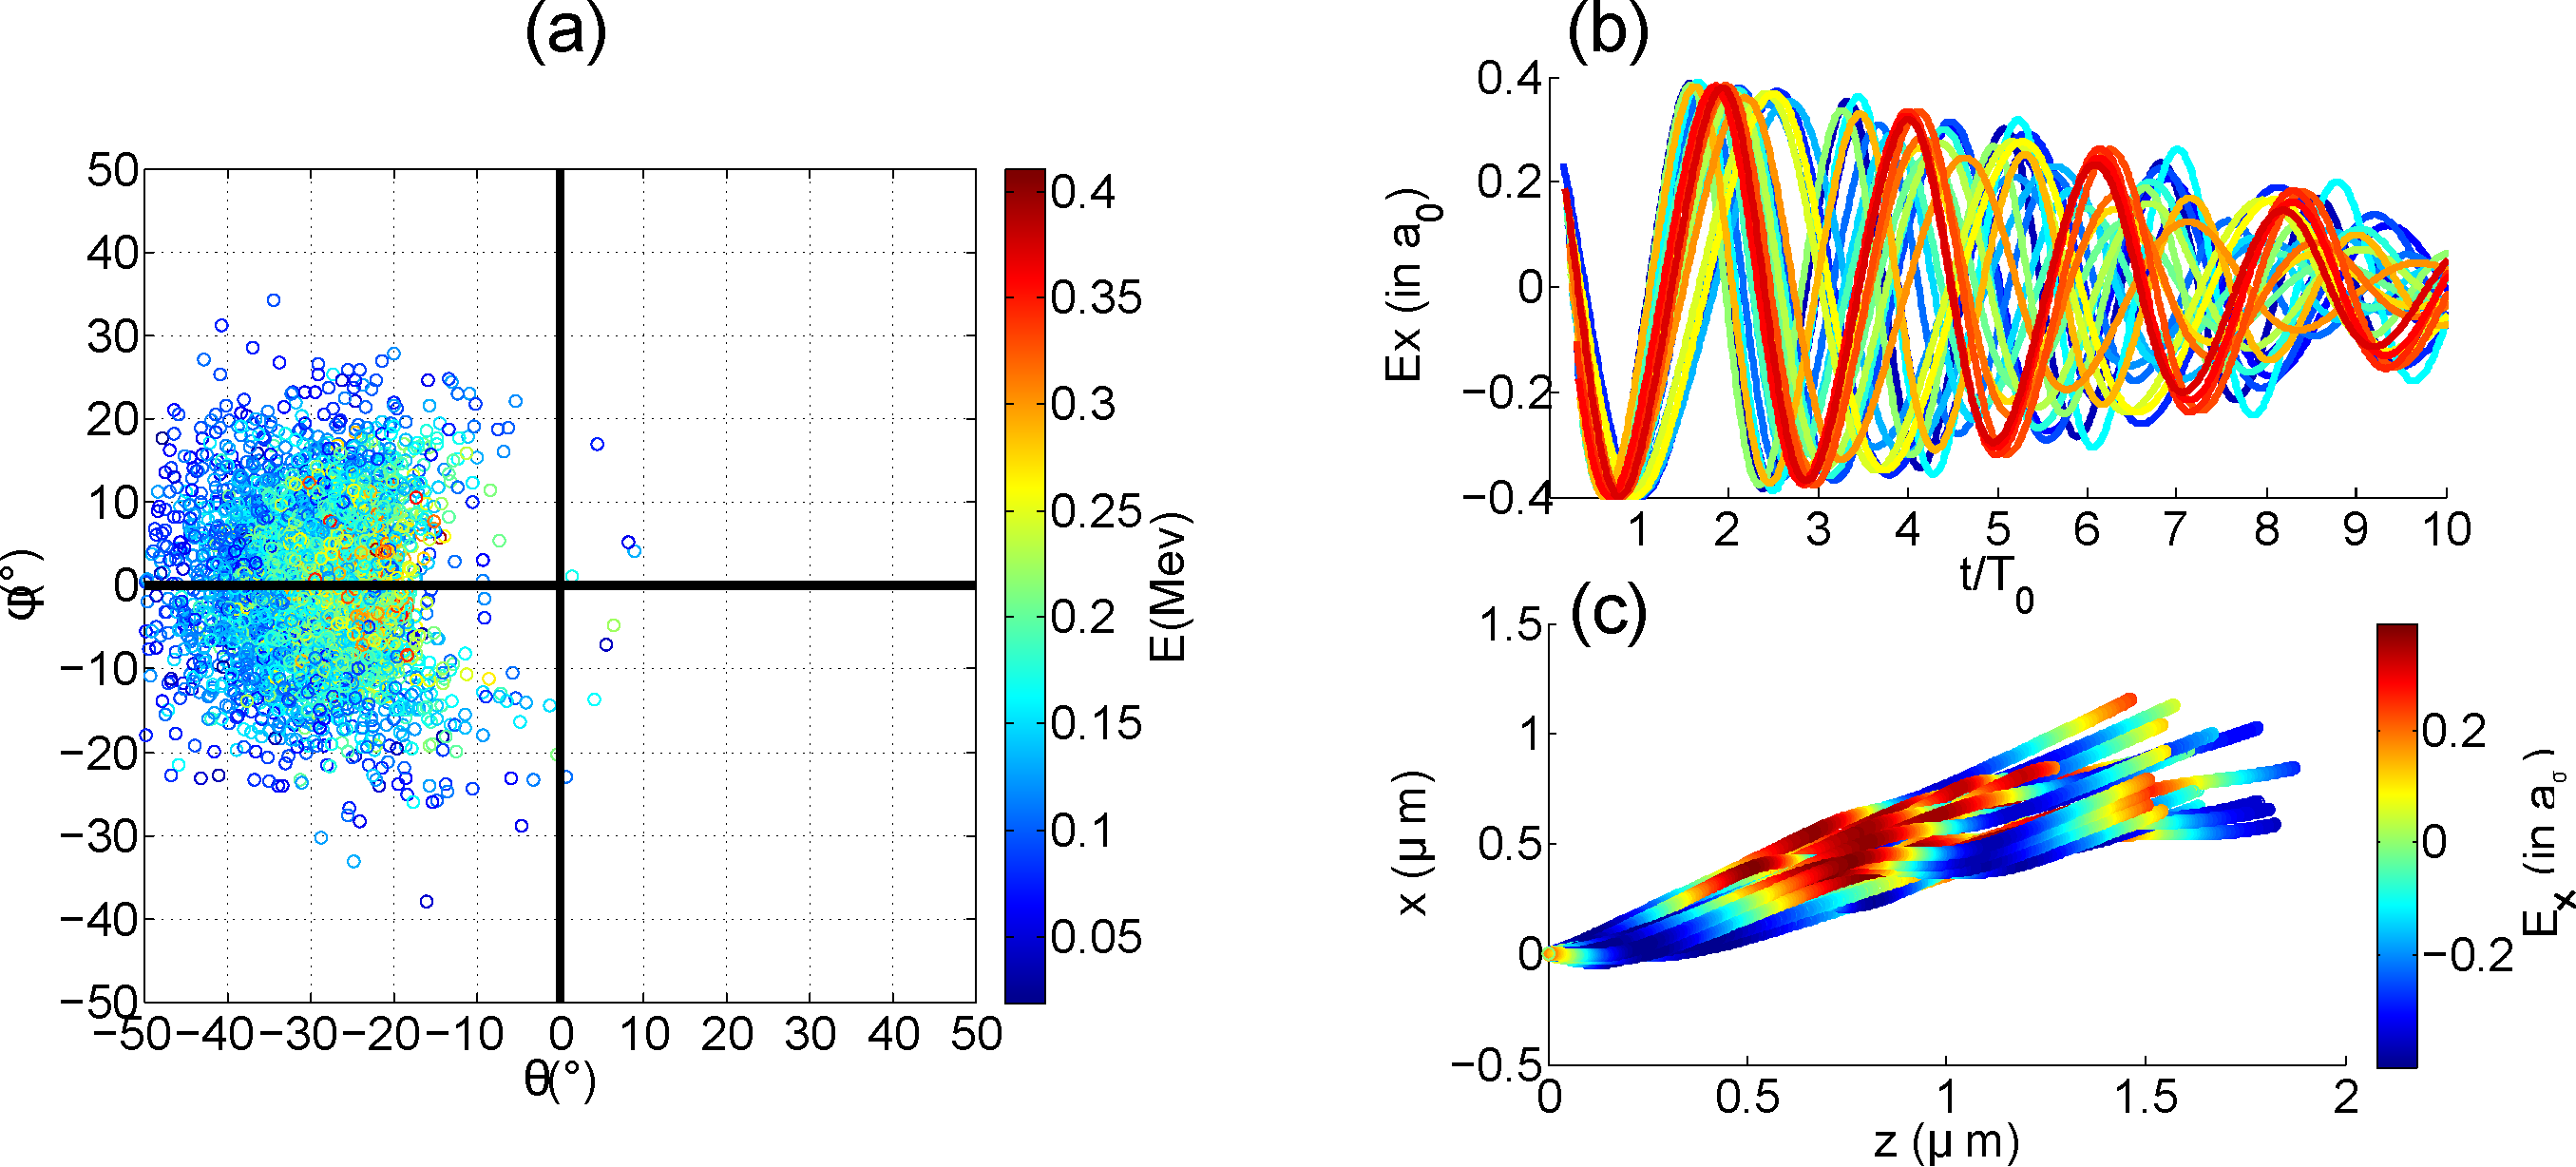
\includegraphics[width =\textwidth]{../chapitre2/images/CompilePhase0.pdf}}
\end{center}
\caption{\label{fig:effectInterferenceSubRelativistic}(a) Final electron angular profile. The final energy is indicated by the colorbar. The solid cross indicates the direction of propagation (b) Field $E_x$ felt by 25 test electrons from the moment they are injected into the propagating laser at position $(0,0)$. (c) Trajectories of these 25 test electrons. The laser characteristics are $a_0 = 0.4$, $w_0 = 2$. }
\end{figure}

In the sub-relativistic regime, electrons are quickly dephased from the laser as illustrated in Fig~\ref{fig:effectInterferenceSubRelativistic}(b), where we plotted the field actually felt by 25 test electrons inside the laser field during 10 optical cycles. In other words, they will "see" several oscillations of the laser, which means they experience ponderomotive acceleration. However, it is interesting to see from Fig~\ref{fig:effectInterferenceSubRelativistic}(c) how the trajectories, and therefore the final angular distribution, is affected by the initial electron injection phase. 




\subsection{Effect of interference field}\label{subsection:Effet of interference field}

In a solid-target experiment, accelerated electrons that escape the plasma interact with a beam reflecting off the critical surface. This means that the incident and reflected pulse interfere. We wish to estimate the effect of this interference field on the electron acceleration and spatial shaping. We already saw in the description of standard electron acceleration schemes that interference fields can alter the acceleration mechanism (two wave beating, stochastic heating). However, in these schemes the interference field is constructed with long laser pulses in the plane-wave approximation. For short ($\sim \,\mathrm{fs}$) tightly focused ($\sim \lambda$) pulses, it is no longer possible to derive the effect of an interference field using standing plane waves because the electrons can very easily "escape" the field in a time comparable to the laser period. 
We use our 3D particle code to construct the interference field by building a reflection on the target plane now defined by $z=0$ as follows:\\
\begin{itemize}
\item[$\bullet$] Two laser beams are added with intensities $a_{01}$ and $a_{02}$, respectively. For construction, we impose $a_{01} = a_{02} = a_0$. The respective $\g{k}$ vector directions are obtained by rotating the vector $(0,0,1)$ by respectively $\theta_1 = -3\pi/4$ and $\theta_2 =-\pi/4$ in the (x,z) plane. This leads to $\g{k}_i \propto (-1,0,-1)$ and $\g{k}_r \propto (-1,0,1)$ as represented in Fig~\ref{fig:interferenceFieldConstruction}.
\begin{equation}
  \left\{
      \begin{aligned}
      \left( \begin{array}{c}
E_{x} \\
E_{z}  \end{array} \right)_r= 
 \left( \begin{array}{cc}
\cos (\theta_1) & \sin(\theta_1)\\
-\sin(\theta_1) &  \cos (\theta_1)   \end{array} \right) \left( \begin{array}{c}
E_0 \\
0  \end{array} \right)
      \end{aligned}
    \right.
\end{equation}
\begin{equation}
  \left\{
      \begin{aligned}
      \left( \begin{array}{c}
E_{x} \\
E_{z}  \end{array} \right)_i= 
 \left( \begin{array}{cc}
\cos (\theta_2) & \sin(\theta_2)\\
-\sin(\theta_2) &  \cos (\theta_2)   \end{array} \right) \left( \begin{array}{c}
E_0 \\
0  \end{array} \right)
      \end{aligned}
    \right.
\end{equation}


\item[$\bullet$]  The field is taken equal to zero in the region $z<0$.
\item[$\bullet$]  Electrons are injected at a given phase of the reflected laser from plane $z=0$. Because of the angle of incidence, this implies the relation 
$$
t_{in} + \frac{x\sin(\pi/4)}{c} = constant
$$
\end{itemize}
Of course, this way of constructing the reflection ultimately leads the field to verify the limit condition of a perfect reflection at the interface $z=0$. This indicates our plasma mirror is represented by a perfect conductor with absolute optical flatness. 
However, the experimental observation of surface plasmons on plasma mirror (section~\ref{section:Review of electron acceleration mechanisms},~\cite{fedeli2015electron}) for uncontrolled gradient length is an indication that the perfect reflector approximation becomes false when increasing the gradient scale length. 


\begin{figure}[H]
\begin{center}
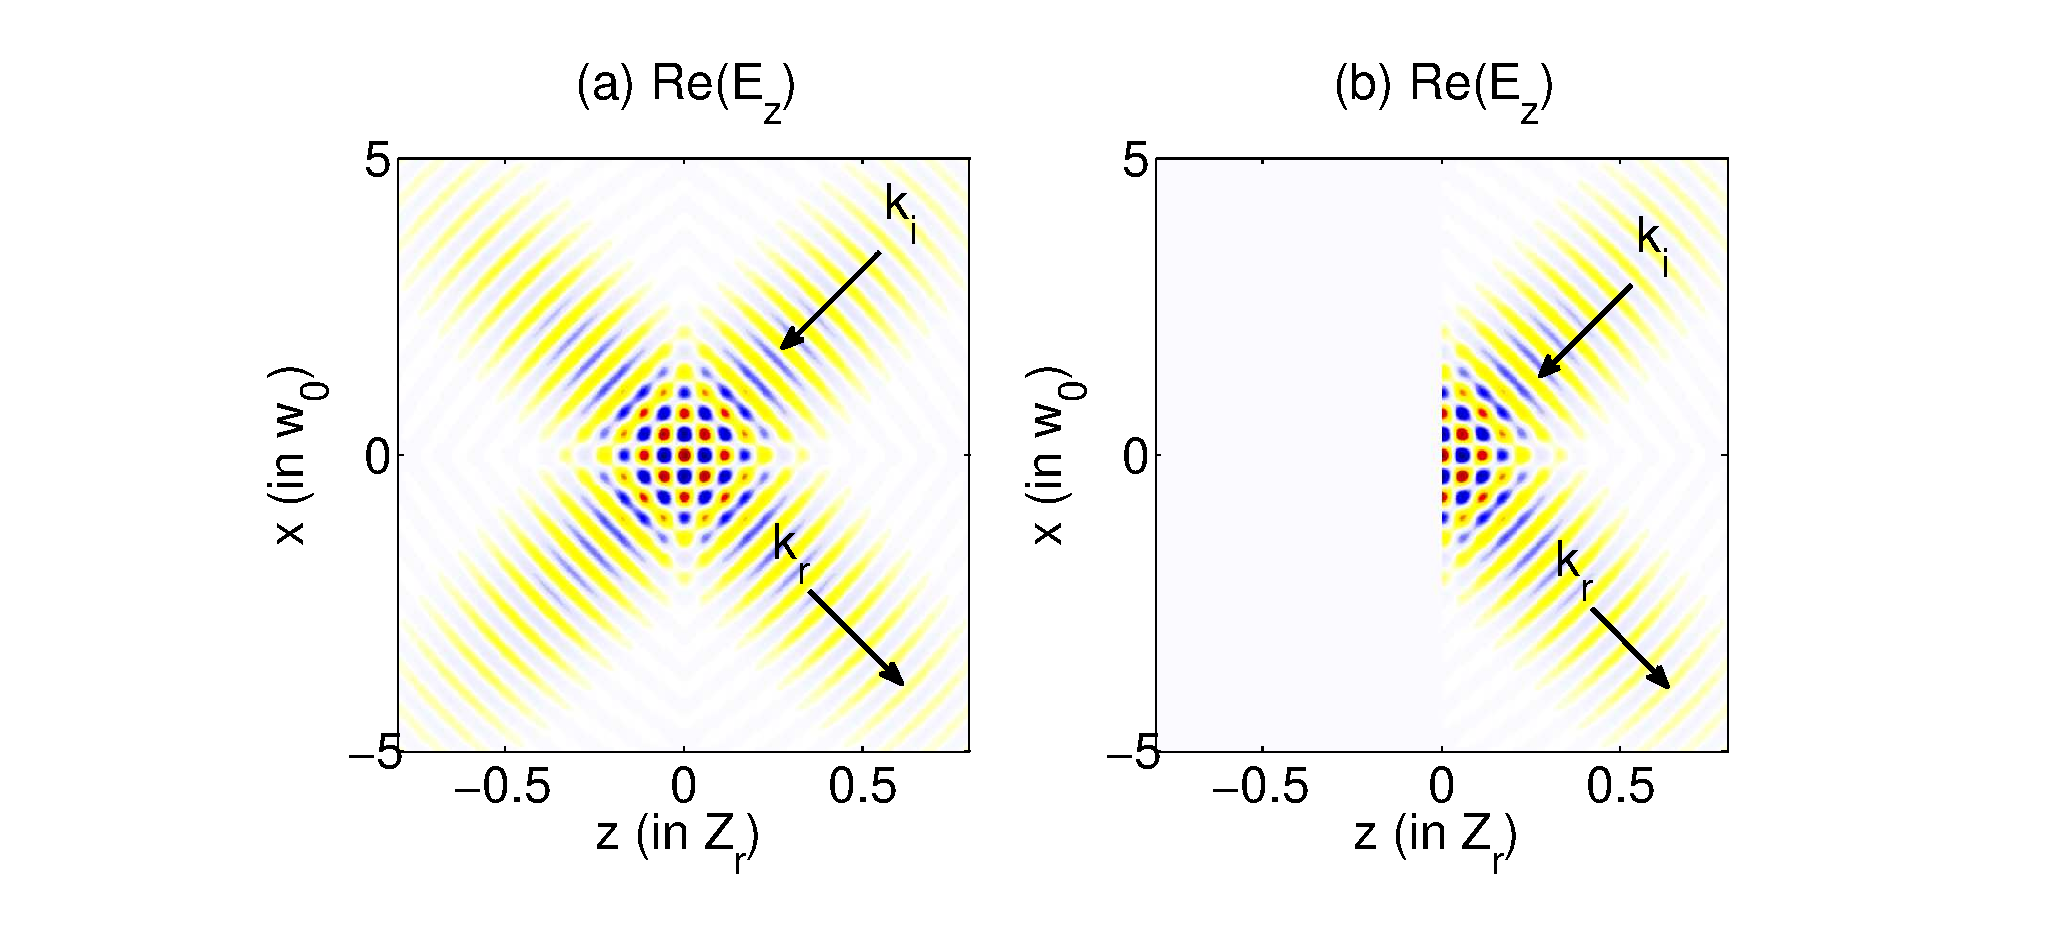
\includegraphics[width =\textwidth]{../chapitre2/images/interferenceFieldConstruction.pdf}
\caption{\label{fig:interferenceFieldConstruction} (a) Incident and reflected pulses are propagating in directions respectively $k_i$ and $k_r$ with respective intensities $a_{01}$ and $a_{02}$. We then impose the field to be equal to zero in the region $z < 0$.}
\end{center}
\end{figure}
%
%\begin{figure}[H]
%\begin{center}
%\makebox[\textwidth][c]{
%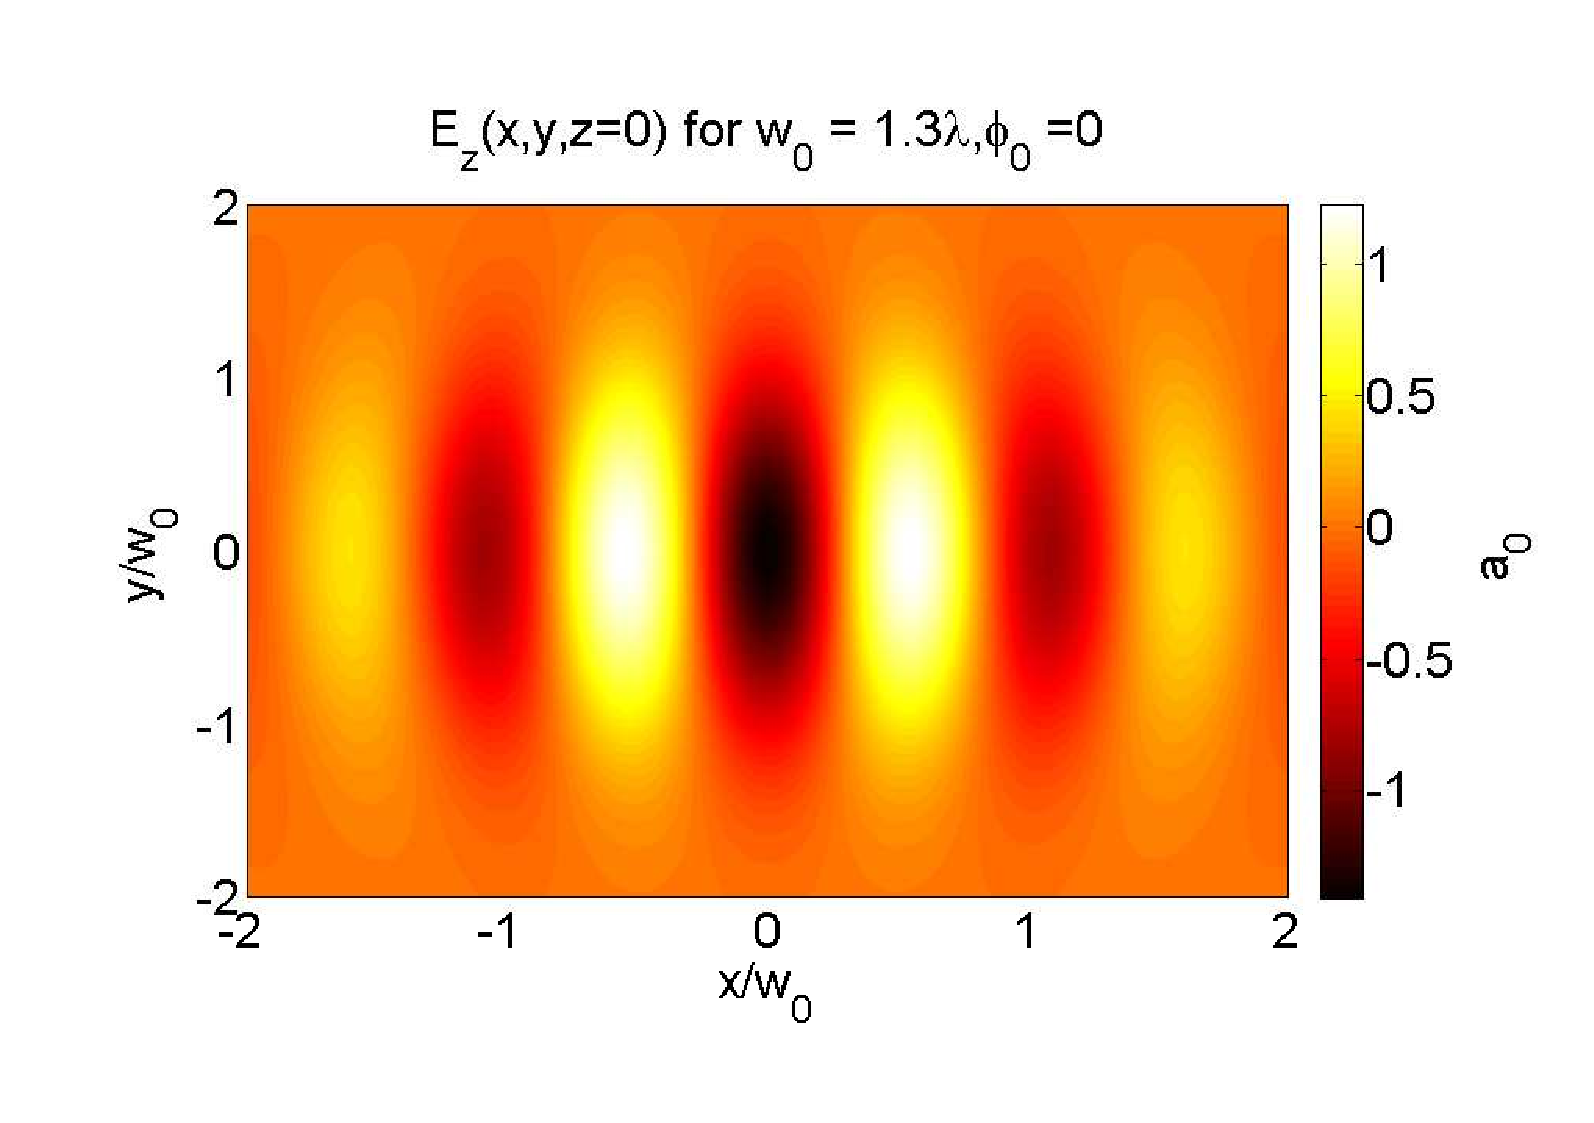
\includegraphics[width =8cm]{../chapitre2/images/Ez_interfrence_w0=1_30fs_phi=0.pdf}
%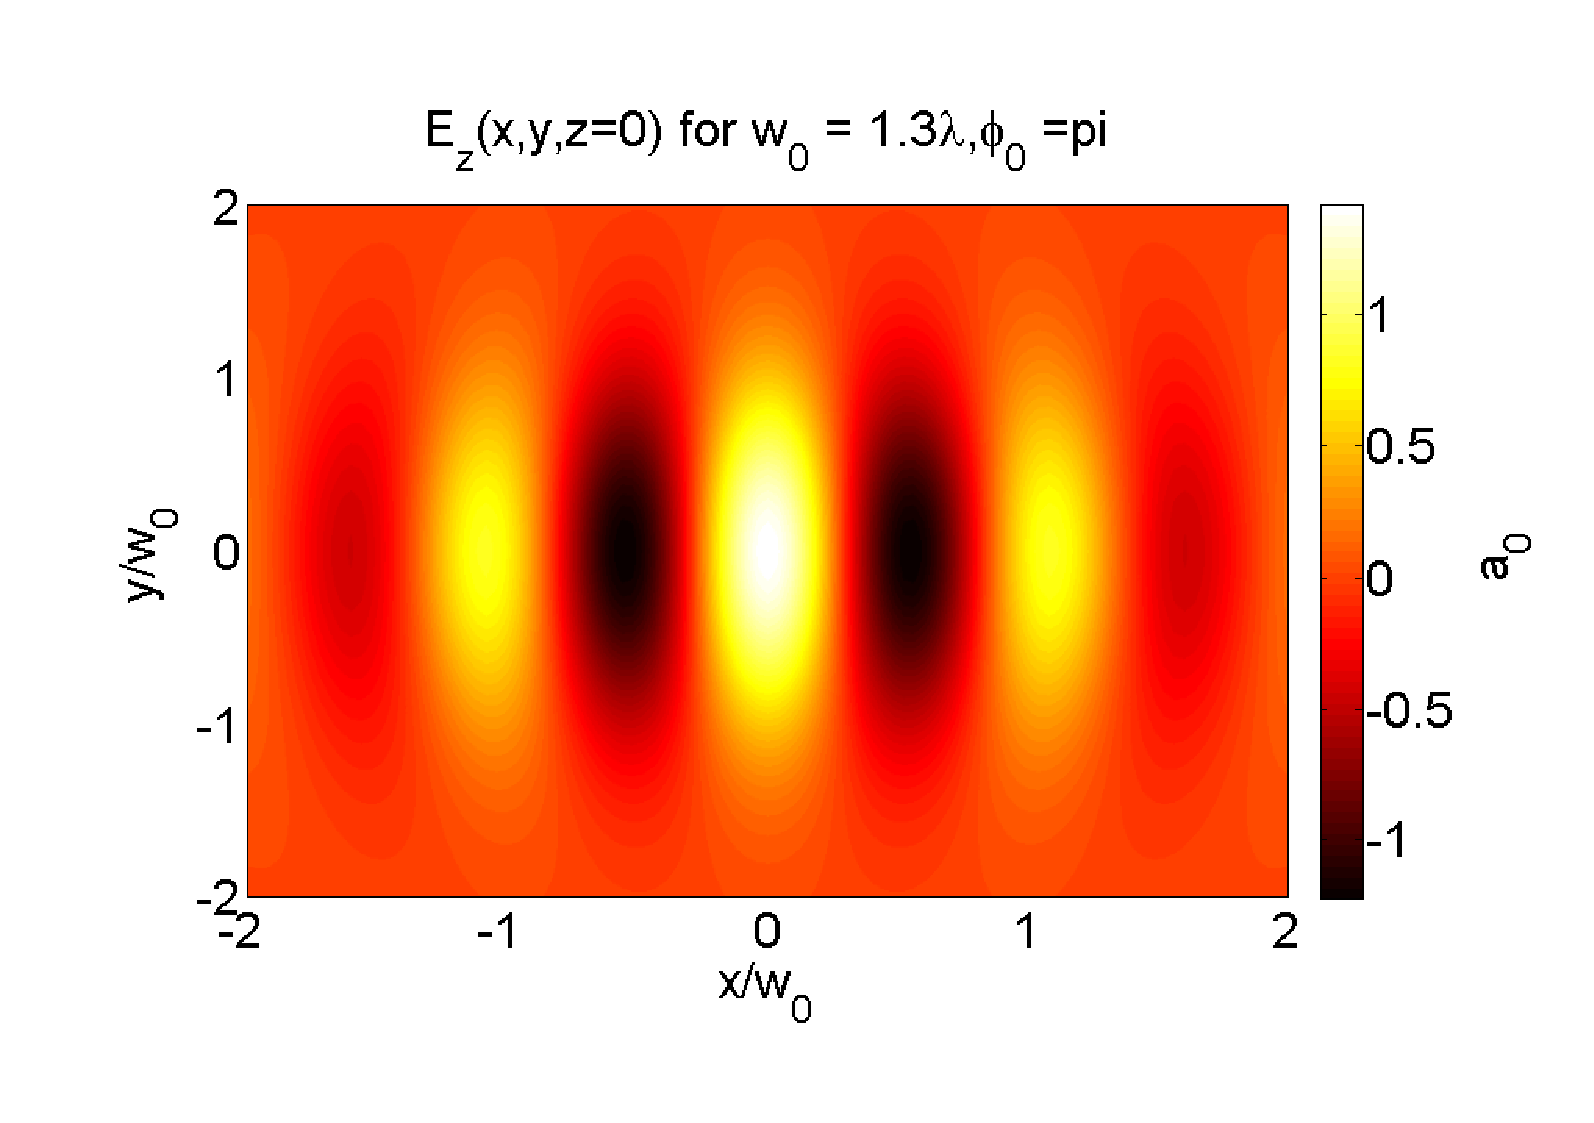
\includegraphics[width =8cm]{../chapitre2/images/Ez_interfrence_w0=1_30fs_phi=3p14.pdf}}
%\caption{\label{fig:Ez-withInterferences} Representation of normal component of the electric field at $t=0$ on the reflecting surface for an absolute phase (CEP) of respectively $0$(left) and $\pi$(right) . One can see the symetrie with respect to plane $y = 0$}
%\end{center}
%\end{figure}

\noindent Once this field has been constructed, we can inject test particles into the interference field from the plane $z=0$ at any given time $t_{in}$ and calculate their trajectories in order to evaluate to possible influence of the interferences ($a_{02}\ne 0$) on both the spatial and spectral properties of the electron beam. In particular, we wonder whether (i) electrons can gain energy in the laser pulse (ii) if electrons can get trapped into the field to be efficiently accelerated.\\

\noindent Note that for the reflected field only, injecting test electrons at a constant phase $\phi_r$ of the reflected laser beam corresponds to:
$$
\g{k}_r\g{r} - \omega_0 t = \phi_r
$$

\noindent and for the incident beam:

$$
\g{k}_i\g{r} - \omega_0 t =\phi_i
$$

\noindent Therefore, injecting electrons at a given time into the interference pattern, we have $\phi_i  - \phi_r = (\g{k}_i - \g{k}_r)\g{r}$. In the case of perfect reflection, this implies $\phi_i = \phi_r$ on a surface parallel to the target, which means a constant phase of the reflected beam is also a constant phase of the incident beam.


\begin{figure}[H]
\begin{center}
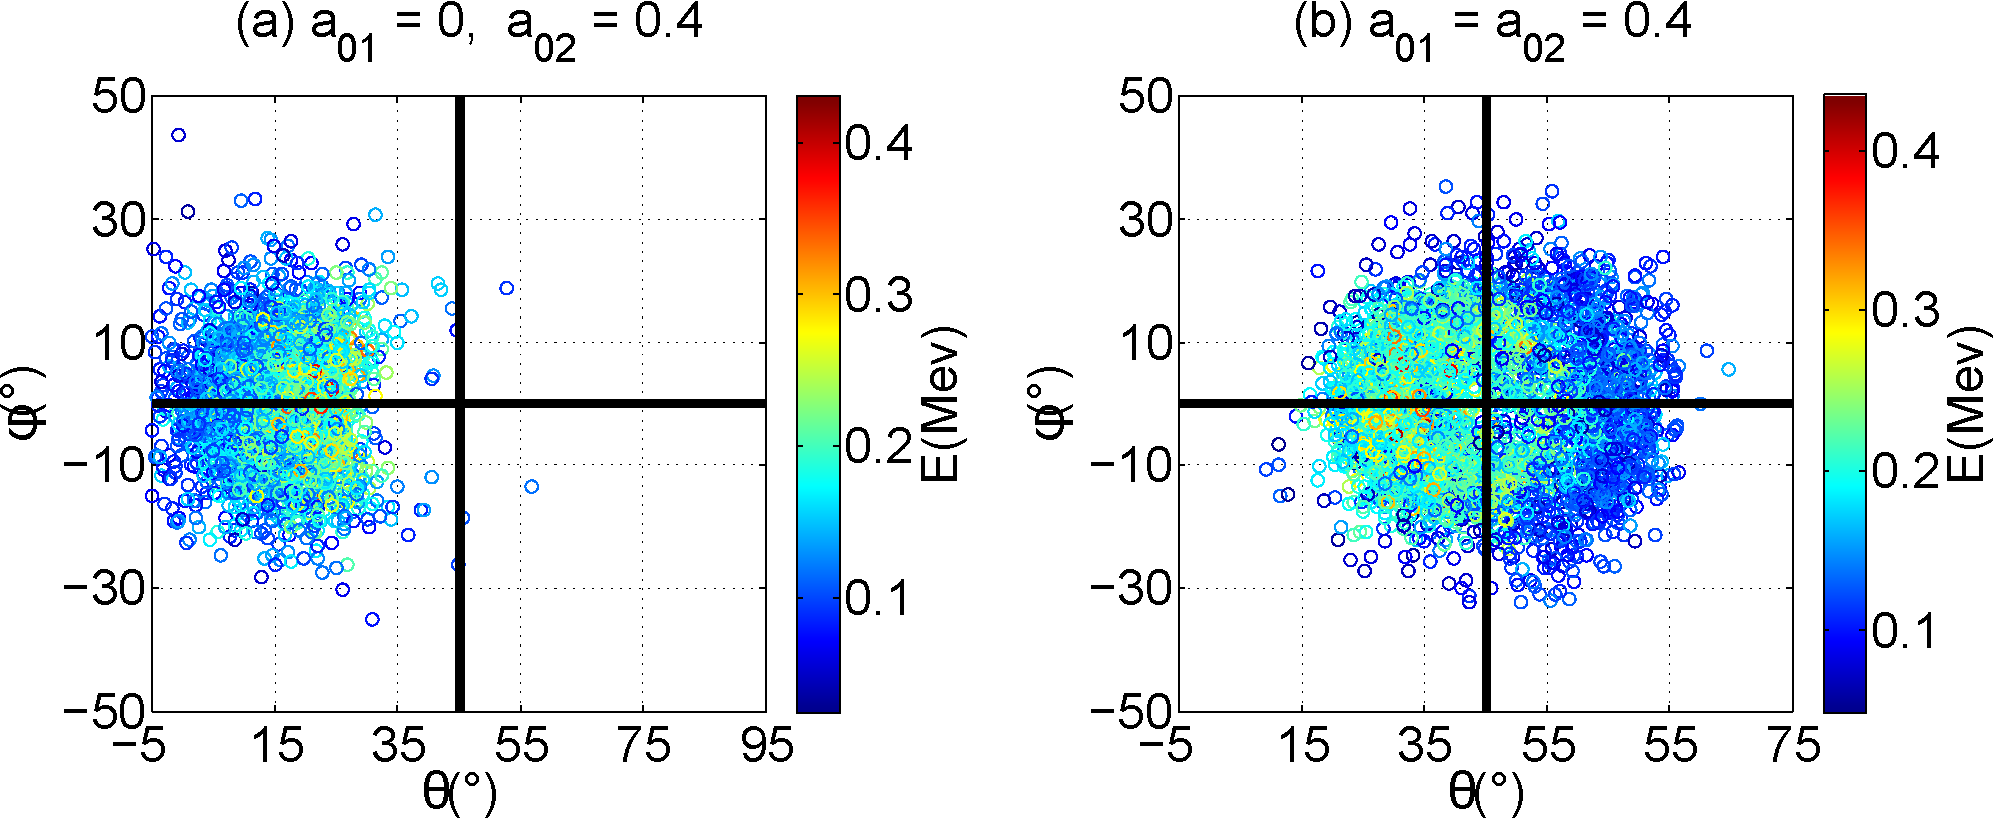
\includegraphics[width =\textwidth]{../chapitre2/images/EffectInterferencesa0=0p4.pdf}
\end{center}
\caption{\label{fig:SumUpa0=1_w0=3} Final angular distribution of electrons for $a_0 = 0.4$ with(b) and without(a) incident field}
\end{figure}

\noindent The ejected electrons are much closer to the specular direction when taking into account the incident laser. This can be well understood for the case of perfect reflection on the surface $z=0$, where the electric field is along the target normal only, thereby reducing the initial canonical momentum of the electron in the direction $x$ along the target surface.


\noindent When taking into account the incident field, the components $E_x$ and $B_z$ vanish in the plane of reflection $z=0$ because of the perfect reflector hypothesis. This is equivalent to reducing the initial canonical momentum towards $\theta <0$ values. We expect the electron angular profile closer to the specular direction, which is indeed the case in our experiment. 

\subsection{Non-axis-symmetrical components of the interference field}\label{sub:Influence of non axisymmetrical component of the interference field}

In section~\ref{subsub:Spatial distribution of ejected electrons}, we mentioned the appearance of $\phi =0$ as a plane of symmetry for the electron angular emission profile. In particular, this profile is shown in Fig~\ref{fig:a0_depletionEffect} for laser intensities of respectively $a_0 = 0.7$ and $a_0 = 1$.

%\begin{figure}[H]
%\centering
%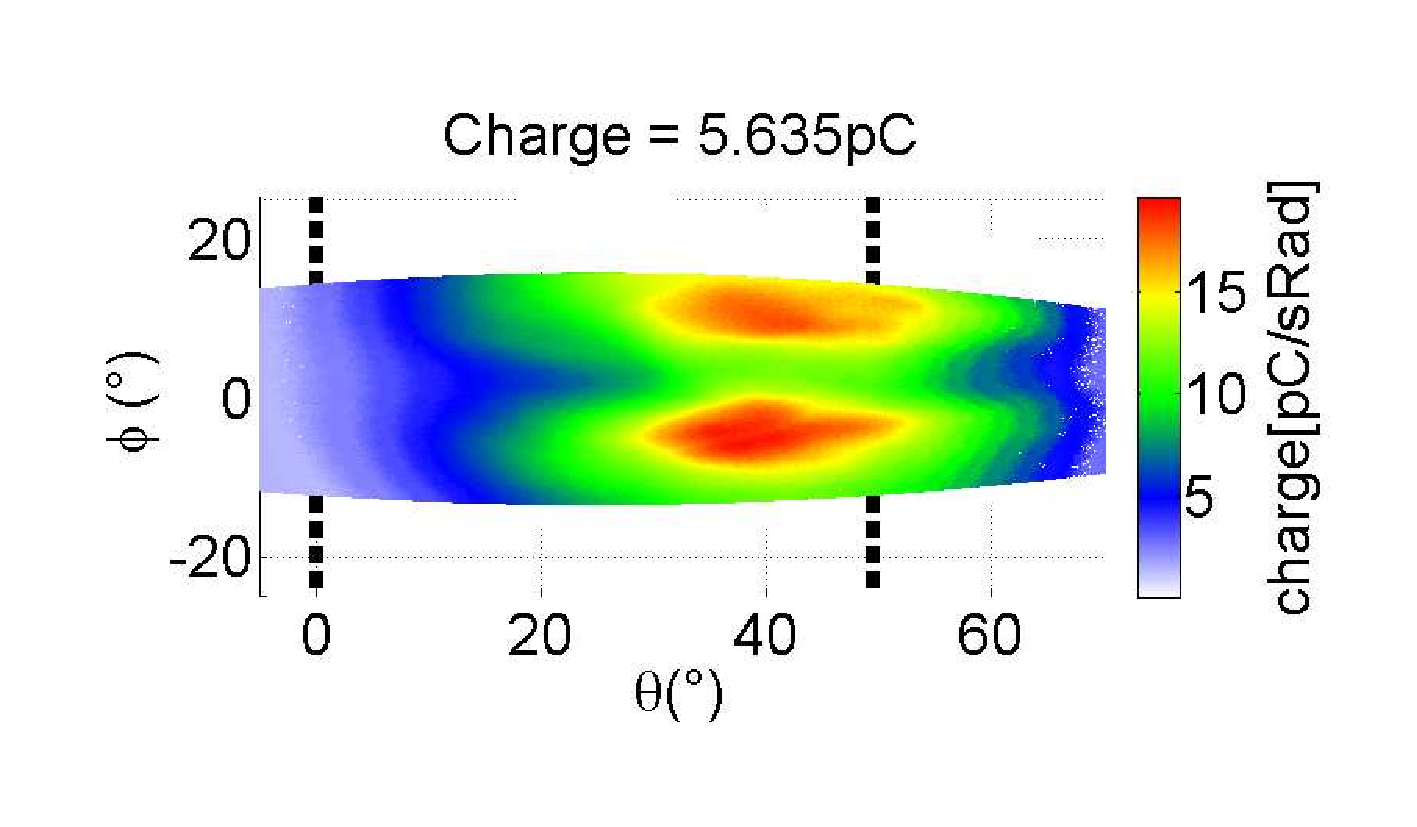
\includegraphics[width =\textwidth]{../chapitre4/images/focus-20-tir220-227.pdf}\\
%\caption{\label{fig:focus-20-tir220-227} Representative experimental electron distribution in the plane of laser polarization for an intensity on target $a_0 = 0.77$ and a focal spot of waist $w_0 = \mathrm{2.7 \mu m}$ }
%\end{figure}


\begin{figure}[H]
\centering
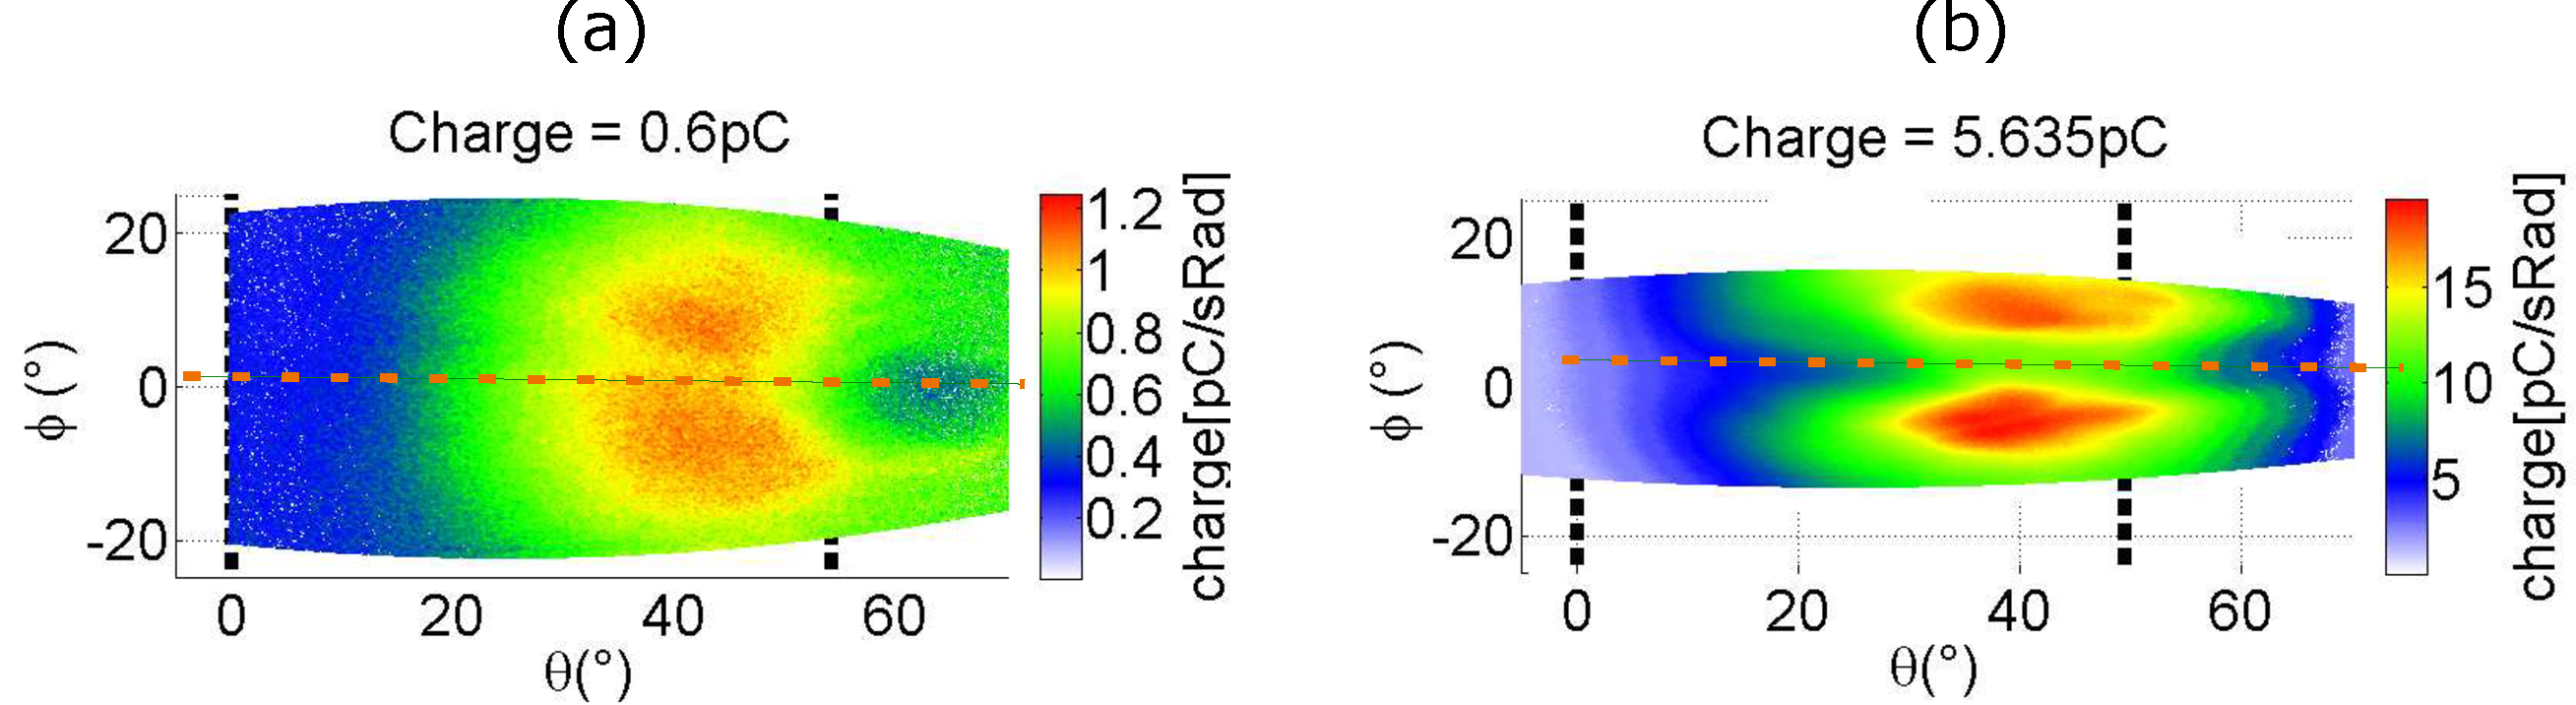
\includegraphics[width =\textwidth]{../chapitre2/images/a0_depletionEffect.pdf}\\
\caption{\label{fig:a0_depletionEffect} Experimental angular emission profile (a) $a_0 \sim 0.7$ (b) $a_0\sim 1$}
\end{figure}

The appearance of the depletion line indicated by the dotted orange line in Fig~\ref{fig:a0_depletionEffect} can be understood by looking at the symmetry of the $B_x$ component still remaining from the interference field, represented in Fig~\ref{fig:FieldProfiles_xyPlane}(b). Indeed, in the target plane, the upper part ($y>0$) of the electrons "feel" a magnetic field $B_x$ of opposite sign from that of the lower part ($y<0$). Considering the $-e \g{v}_z\times \g{B}_x = -ev_zB_x \g{u}_y$ component, and assuming $v_z>0$, the force is directed upward when $B_x<0$ and downward when  $B_x >0$. This symmetry argument could explain why we observe, at high intensity and in a tight focusing configuration (Fig~\ref{fig:a0_depletionEffect}(b)), a depletion line in the angular profile rather than a simple ponderomotive hole. Note that without the first-order decomposition of the field with respect to parameter $\epsilon = \frac{\lambda_0}{2\pi w_0}$, we would have $B_x$ rigorously equal to $0$, and we could thus not explain our observations.\\

\noindent Based on Fig~\ref{fig:FieldProfiles_xyPlane}, and considering only the zeroth order term of the electromagnetic field (paraxial approximation), the equation of motion in the laboratory referential is written (the component which have disappeared because of the interference field are indicated in \textcolor{red}{red color}):

\begin{subequations}
\label{eq:EquationGyro-1}
\begin{align}[left = \empheqlbrace\,]
&\frac{d}{dt}[\gamma v_x] =- \frac{e}{m_e}\textcolor{red}{E_x} + \frac{e}{m_e}v_zB_y=- \frac{e}{m_e}\frac{E_0}{\sqrt{2}}(\textcolor{red}{1} - 2\sqrt{2}\frac{v_z}{c}) \label{gyro-1} \\
&\frac{d}{dt}[\gamma v_z] =- \frac{e}{m_e}E_z - \frac{e}{m_e}v_xB_y=- \frac{e}{m_e}\frac{2E_0}{\sqrt{2}}(1 + \sqrt{2}\frac{v_x}{c})  \label{gyro-3} 
\end{align}
\end{subequations}

\noindent Which, using the normalizing conventions of Appendix~\ref{ch:Normalisation conventions} we have:

\begin{subequations}
\label{eq:EquationGyro-norm}
\begin{align}[left = \empheqlbrace\,]
&  \frac{d}{d\bar{t}}[\gamma v_x] =- \frac{1}{\sqrt{2}}\frac{\omega_{ce}}{\omega_0}(\textcolor{red}{1} - 2\sqrt{2}v_z)=2 \frac{\omega_{ce}}{\omega_0}v_z \label{gyro-1} \\
&   \frac{d}{dt}[\gamma v_z] =- \frac{2}{\sqrt{2}}\frac{\omega_{ce}}{\omega_0}(1 + \sqrt{2}v_x)  \label{gyro-3} 
\end{align}
\end{subequations}FTraject




\begin{figure}[H]
\begin{center}
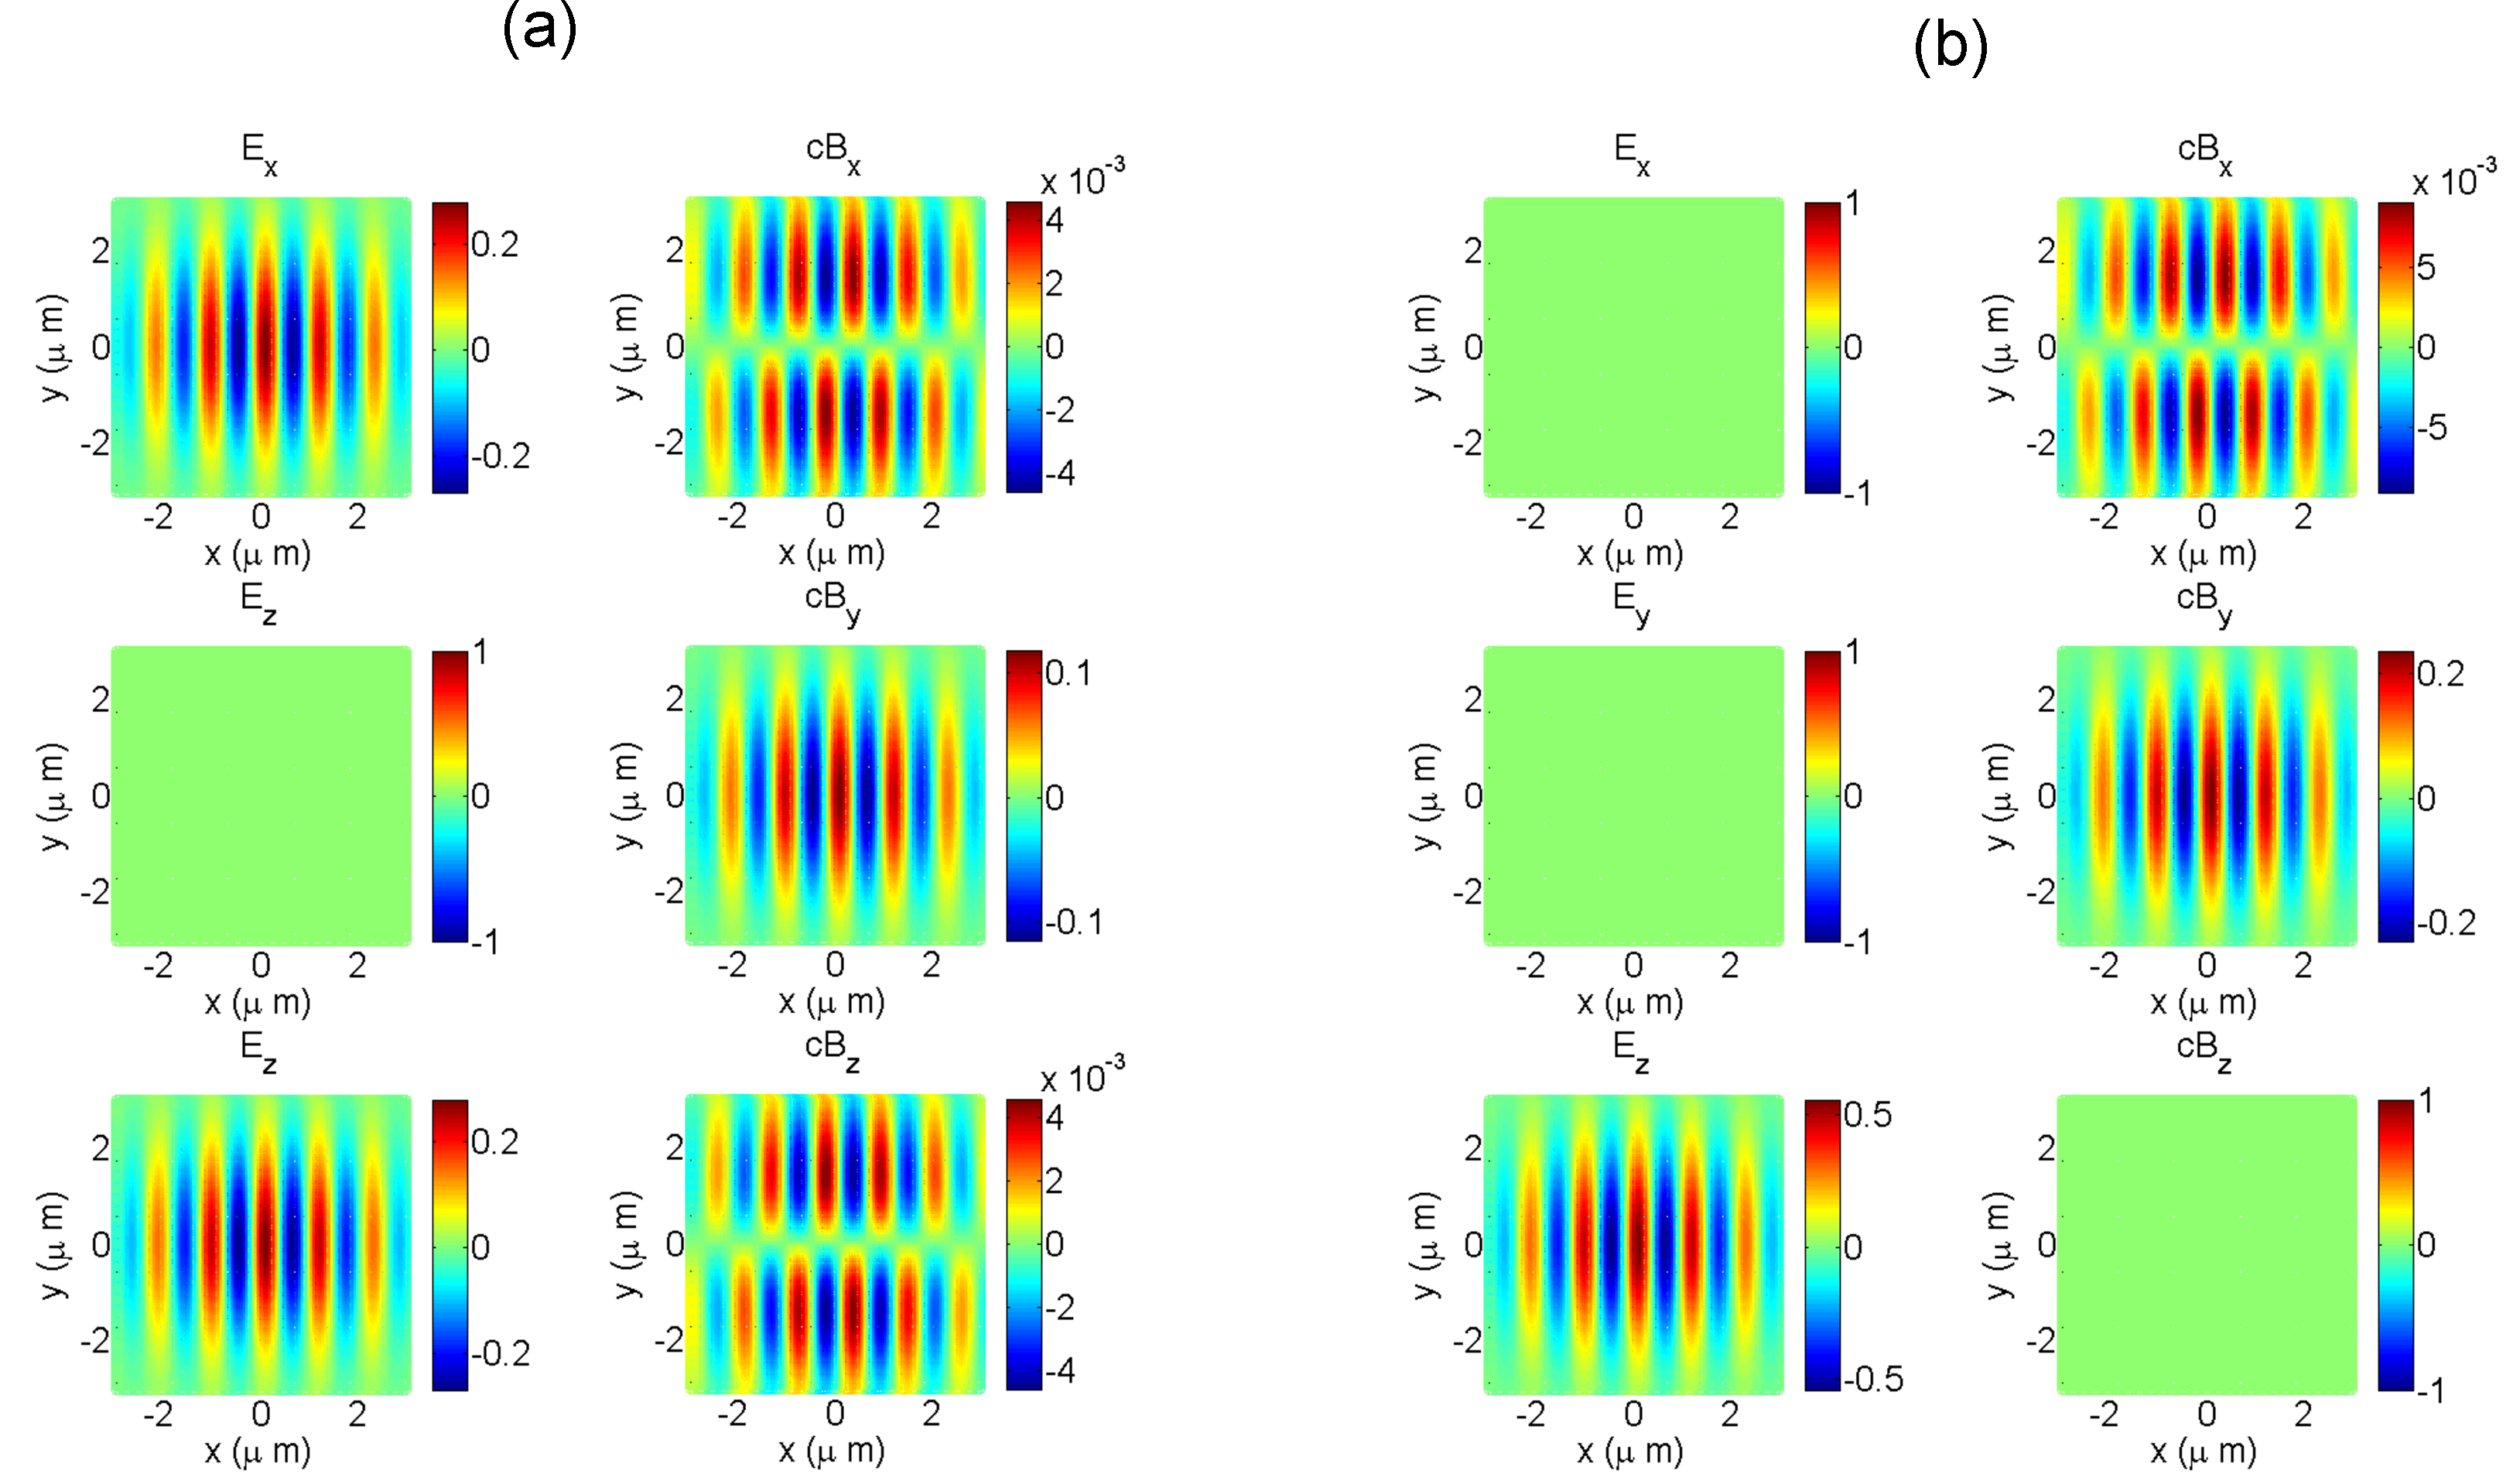
\includegraphics[width =\textwidth]{../chapitre2/images/FieldProfiles_xyPlane.pdf}
\end{center}
\caption{\label{fig:FieldProfiles_xyPlane} Fields  on plane $z=0$ at $t = 0$, with $a_0 = 0.4$, $w_0 = 2$ \textcolor{red}{with} (a) and without (b) incident field at $45^{\circ}$ incident angle}
\end{figure}



\noindent The cancellation of the \textcolor{red}{electric term} relative to the magnetic term in equation~\ref{eq:EquationGyro-norm} leads to the well-described gyromagnetic effect~\cite{geindre2006relativistic}, already introduced in section~\ref{eq:Gyromagnetic confinement for short gradient scale lengths}. Indeed, since the magnetic field does not work, its dominant action will force particles to remain in orbits of constant energy, that is to stay closed orbits near the surface. This effect is all the more pronounced as the intensity is high. This is illustrated by the comparison of Fig~\ref{fig:GyroAndDepltetion_a0effect} (b) and (c), where test electrons are injected at a node of the magnetic field along a vertical line $x=0$, with or without interference field. we clearly see in Fig~\ref{fig:GyroAndDepltetion_a0effect} (b) that electrons initially located in the center $y\sim 0$ do not escape the surface.


\begin{figure}[H]
\centering
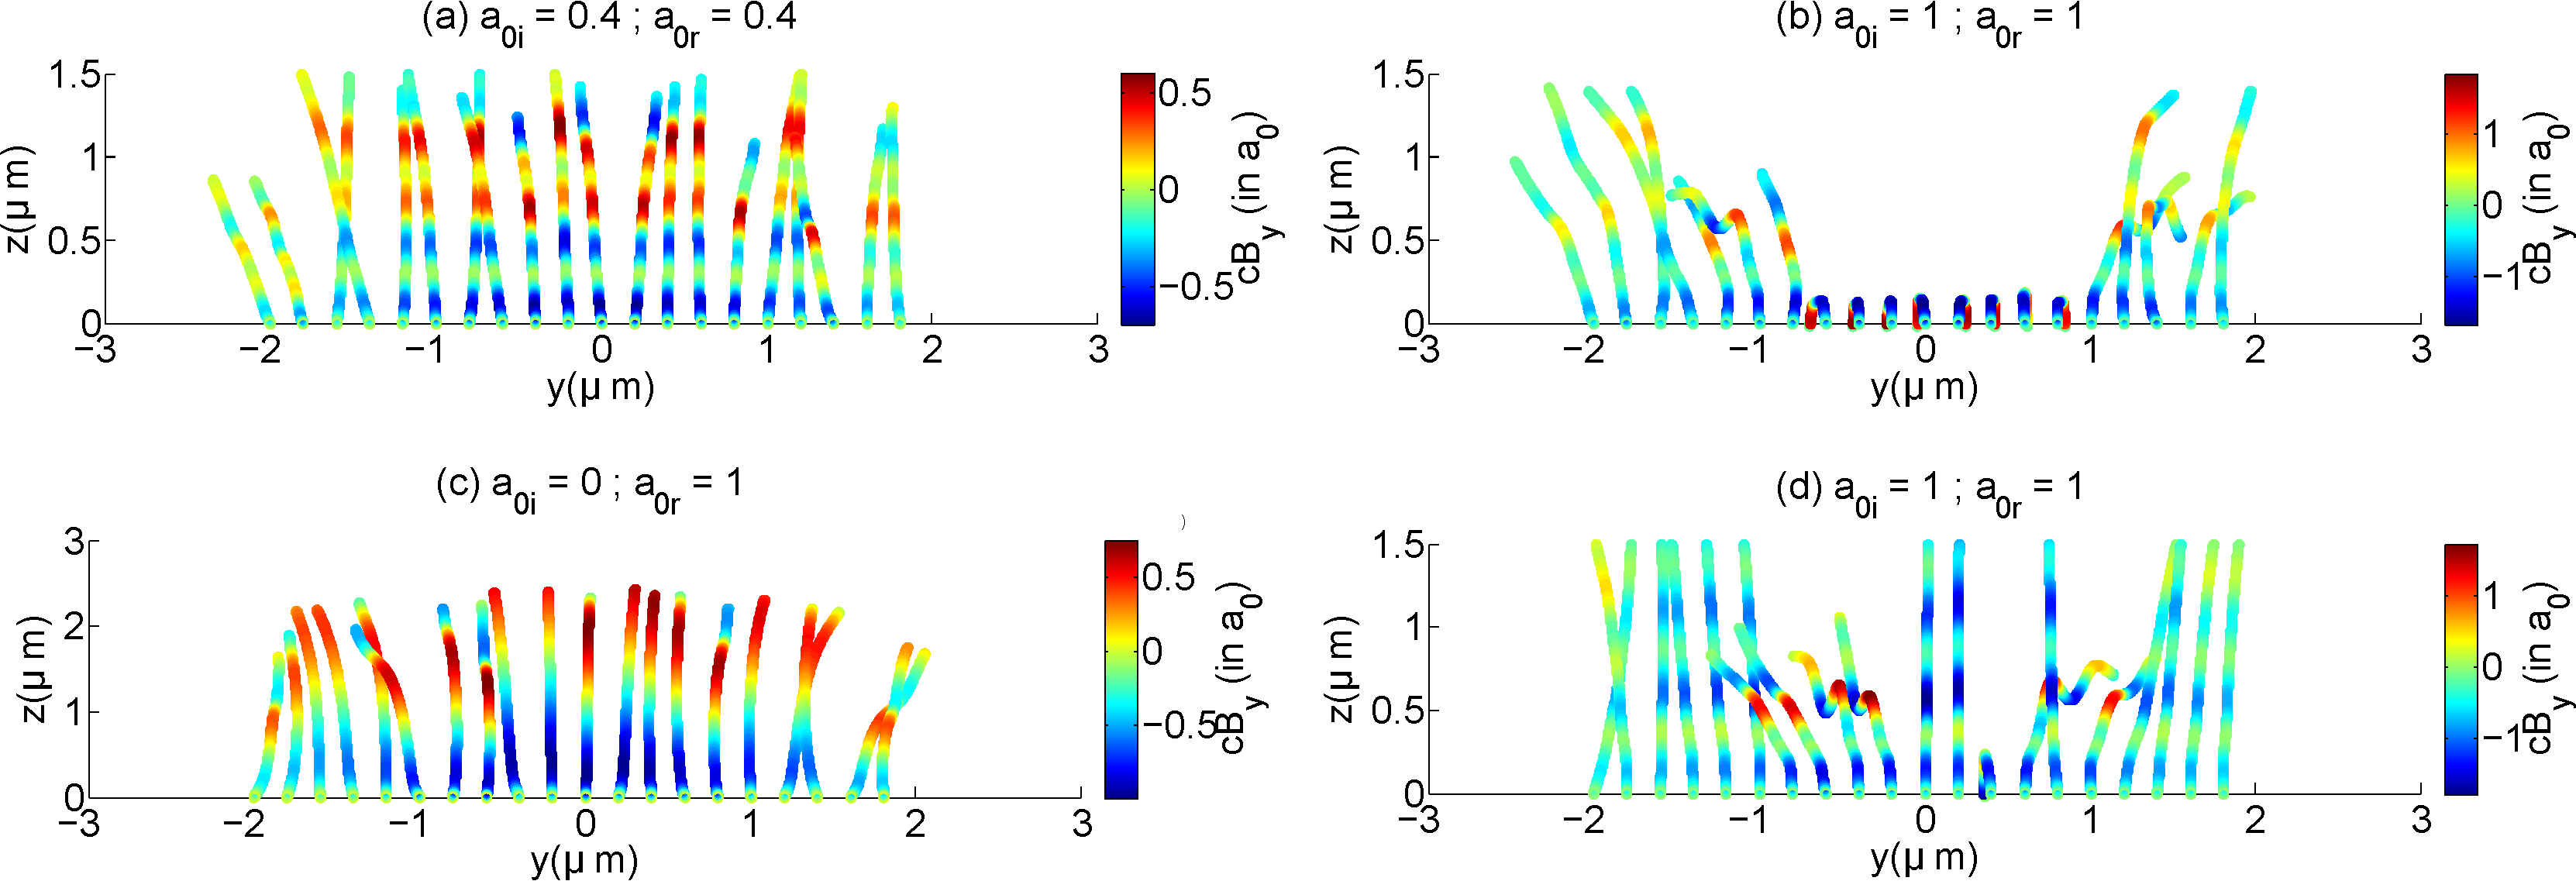
\includegraphics[width =\textwidth]{../chapitre2/images/GyroAndDepltetion_a0effect.pdf}\\
\caption{\label{fig:GyroAndDepltetion_a0effect} Trajectories over $4$ optical cycles of 20 test electrons injected when $B_y$ becomes negative. The color scale indicates the magnetic field $B_y$ felt by the electron over time. Test electrons are positioned along a vertical line $y\in [-w_0 \ ; \ w_0]$. (a) Low-intensity case $a_0 = 0.4$; (b) high-intensity case $a_0 =1$ (c) No interference field, $a_{0r} = 0$ (d) Similar conditions as in (b) when $p_{0z}$ is doubled for all electrons}
\end{figure}









%\begin{figure}[H]
%\centering
%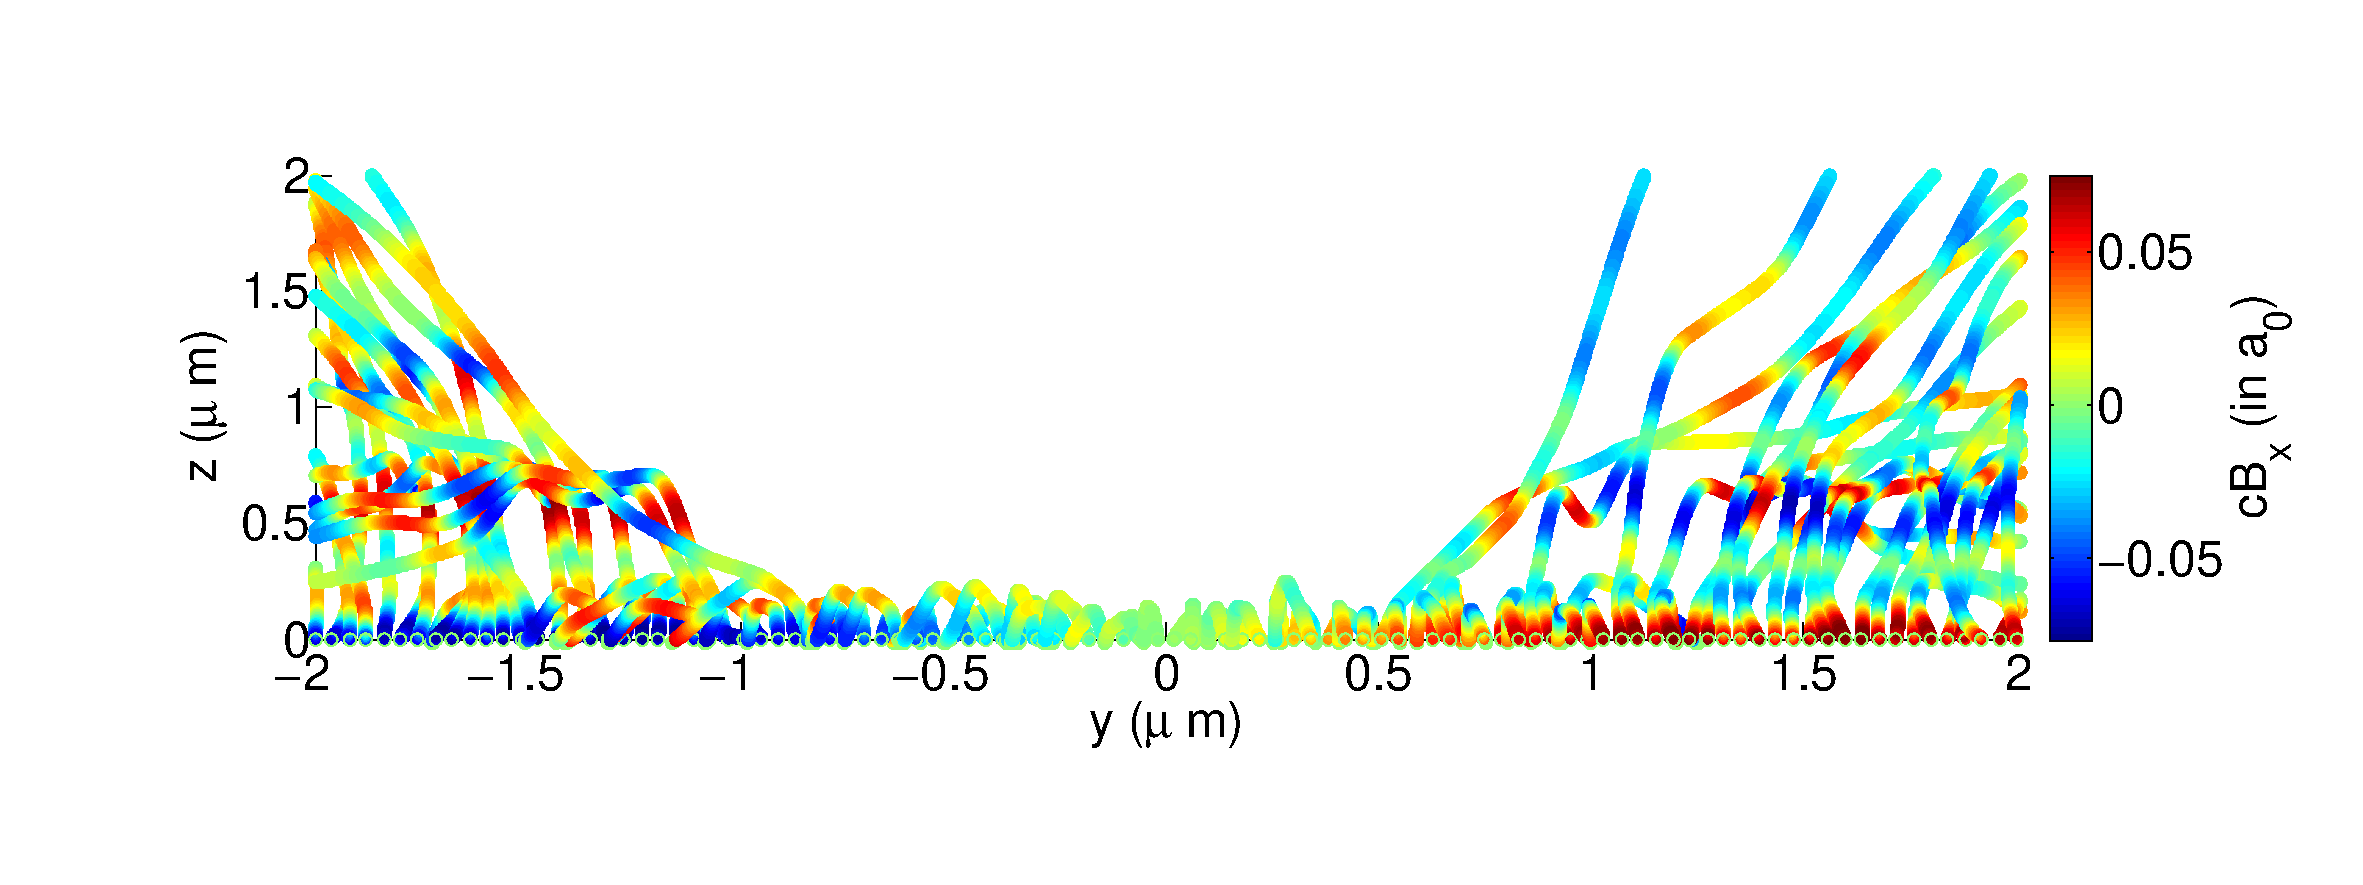
\includegraphics[width =\textwidth]{../chapitre2/images/a0=1_trajectories.pdf}\\
%\caption{\label{fig:a0=1_trajectories}magneetic forcal calls back electrons,$a_0 =1$}
%\end{figure}
%
%We have less particles that can escape because of the gyromagntic effect. The effect will be all the more pronounced that $\g{v}_x\times$ B_y$ has a large value, that is to say 
%


\section{Conclusion}

We have presented two regimes of acceleration, which we call respectively "ponderomotive" and "non-ponderomotive" regimes. In the first case, electrons are expelled by the laser through the ponderomotive force, and a hole is visible in the final electron angular profile. This regime is dominant at sub-relativistic intensities. When the laser intensity is clearly relativistic, as demonstrated in the literature, electrons can be "trapped" in the laser where they are efficiently accelerated. However, we have observed other singular patterns in the electron angular emission profile such as the appearance of a depletion line along the polarization plane. Using a 3D particle code which accounts for the high-order components of the fields in focus, and taking into account the reflection of the field (mostly valid for short gradient scale length) on a planar surface, it was possible to qualitatively reproduce the electron angular emission profiles obtained experimentally. Indeed, the $j\times B$ force is oriented differently depending of the initial position of the electron with respect to the polarization plane. Provided that electrons are confined because of the gyromagnetic effect, this depletion line becomes visible. This experiment will be reproduced at $5\,\mathrm{fs}$ in the near future, and further investigations still need to be made to fully understand the dynamic of the electron-laser interaction in vacuum. 


















